%---------------------------------------------------------------------------%
%---------------------------------------------------------------------------%
%                          MPT THEME - EXAMPLE                              %
%---------------------------------------------------------------------------%
%---------------------------------------------------------------------------%

%---------------------------------------------------------------------------%
% HEADER                                                                    %
%---------------------------------------------------------------------------%

%----- DOCUMENT TYPE--------------------------------------------------------%
%---------------------------------------------------------------------------%

\pdfminorversion = 5
\documentclass[10pt]{beamer}
\usetheme[francais %[For documents written in french]
%,notocfoot %[To remove the presentation title in the footer of the frames]
%,arial %[To use arial as the default text font instead of Linux Biolinum]
,alertred %[For the alterted text to be framed in red instead of blue]
%,euler %[To use euler as the default math font instead of XITS]
%,sober %[To remove the grey areas behind the frame titles and the footer]
]{MPTM} %[Comment and uncomment options as desired]


%----- PACKAGES-------------------------------------------------------------%
%---------------------------------------------------------------------------%
% [Put all desired packages here]

%Notes
\usepackage{pdfpages}
%\setbeameroption{show notes} %[to show note on the pdf]
%\setbeameroption{show notes on second screen=right}%Pour placer les notes à droite, en extension d'une slide mais commande qui ne marche pas


%TIKZ
\usepackage{pgfplots}

\pgfplotsset{compat=1.14}

\usetikzlibrary{calc, 3d, positioning, intersections, backgrounds, shapes, math, shapes.geometric, topaths, decorations.markings, pgfplots.colormaps}
\usepgfplotslibrary{colormaps, fillbetween}
\pgfplotsset{probastyle/.style={smooth, width = \textwidth, axis x line = bottom, axis y line = left,
		every axis x label/.style={ at={(ticklabel* cs:1.05)}, anchor=west,},
		every axis y label/.style={	at={(ticklabel* cs:1.05)}, anchor=south,}}}
\pgfplotsset{ colormap={MPT}{rgb255(0cm)=(0,94,158) rgb255(0.25cm)=(0,111,182) rgb255(1cm)=(240,240,240) rgb255(2cm)=(156,158,159)}}
\pgfplotsset{compat=newest}
\pgfplotsset{school/.style={tick align = outside, major tick length = 2.5pt, axis line style={-stealth}, anchor = center, x label style = {anchor = west, at = {(current axis.right of origin)}}, y label style = {anchor = south, at = {(current axis.above origin)}, rotate = -90}}}
\usepackage{tikz-3dplot}
\tdplotsetmaincoords{60}{-30}
\tdplotsetrotatedcoords{0}{90}{90}
\pgfmathdeclarefunction{gaussShape}{2}{%
  \pgfmathparse{(1/#2)*exp(-((x-#1)^2)/(1^2))}%
  }
  \pgfmathdeclarefunction{gauss}{2}{%
  \pgfmathparse{(1/(#2*sqrt(2*pi)))*exp(-((x-#1)^2)/(2*#2^2))}%
}
\tikzset{
		    base/.style = {draw=MPTgrey, ultra thick, 
			minimum height=30mm, minimum width=30mm,
			inner sep=0pt}, %permet d'afficher une image dans un rectangle
  invisible/.style={opacity=0},
  visible on/.style={alt={#1{}{invisible}}},
  alt/.code args={<#1>#2#3}{%
    \alt<#1>{\pgfkeysalso{#2}}{\pgfkeysalso{#3}} % \pgfkeysalso doesn't change the path
  },
}
\usetikzlibrary{arrows.meta}

%smiley souriant bleu
\newcommand{\smiley}{\tikz[baseline=-0.75ex,black]{
		\draw[MPTblue] circle (2mm);
		\node[MPTblue,fill,circle,inner sep=0.5pt] (left eye) at (135:0.8mm) {};
		\node[MPTblue,fill,circle,inner sep=0.5pt] (right eye) at (45:0.8mm) {};
		\draw[MPTblue] (-145:0.9mm) arc (-120:-60:1.5mm);
	}
}

%smiley pas content rouge
\newcommand{\frownie}{\tikz[baseline=-0.75ex,black]{
		\draw[MPTred] circle (2mm);
		\node[MPTred,fill,circle,inner sep=0.5pt] (left eye) at (135:0.8mm) {};
		\node[MPTred,fill,circle,inner sep=0.5pt] (right eye) at (45:0.8mm) {};
		\draw[MPTred](-145:0.9mm) arc (120:60:1.5mm);
	}
}


%----- MATH
%\usepackage{amsmath, amssymb, amscd, latexsym, bigints, stmaryrd, bm}
\usepackage{stmaryrd, bm}

%----- TABLES
\usepackage{booktabs, tabularx, multirow, colortbl}
\arrayrulecolor{main}
\setlength{\aboverulesep}{0pt}
\setlength{\belowrulesep}{0pt}
\setlength{\extrarowheight}{5pt}
\newcolumntype{L}{>{\raggedright\arraybackslash}X}
\newcolumntype{R}{>{\raggedleft\arraybackslash}X}
\newcolumntype{C}{>{\centering\arraybackslash}X}
\newcolumntype{s}{@{\hspace{3pt}} c @{\hspace{6pt}}}

%----- FIGURES
\usepackage{graphicx, psfrag, color, epsfig}   % to include and manipulate graphics
\usepackage[all]{xy}    % to draw diagrams
%\usepackage{ifsym}
\usepackage{multirow}

%----- LISTS
\usepackage{enumerate}

%----- BIBLIO
\usepackage{bibentry}

%-----BARRER
\usepackage{soul}

%----- SYMBOLS
\usepackage{pifont}
\usepackage{bclogo}

%----Font
\usepackage{verbatim}
\usepackage{fancyvrb}
\makeatletter
\newcommand{\verbatimfont}[1]{\renewcommand{\verbatim@font}{\ttfamily#1}}
\makeatother

%\usepackage{secdot}
%\sectiondot{subsection}

%----- ADDITIONAL COMMANDS 
%---------------------------------------------------------------------------
\newcommand{\bfun}{\bm{1}}
%\let\sectionOld\section
%\renewcommand\section[2][\empty]{%boldmath\sectionOld[#1]{#2}\unboldmath%}
% [Put all user-defined commands here]

%----- Symbols
\newcommand{\ex}{{\color{MPTblue}\ding{228}}}
%\newcommand{\ex}{{\color{MPTblue}\small{\blacktriangleright}}}

%----- SPACES
\newcommand{\hsp}{\hspace*{1em}}
\newcommand{\midhsp}{\hspace*{.5em}}

\makeatletter
\define@key{beamerframe}{c}[true]{% centered
	\beamer@frametopskip=0pt plus 1fill\relax%
	\beamer@framebottomskip=0pt plus 1fill\relax%
	\beamer@frametopskipautobreak=0pt plus .4\paperheight\relax%
	\beamer@framebottomskipautobreak=0pt plus .6\paperheight\relax%
	\def\beamer@initfirstlineunskip{}%
}
\makeatother



%----- BIBLIO
\newcommand{\itbib}[1]{{\itshape \bibentry{#1}}}
%\providecommand{\bysame}{S.I. Resnick}%

%----- PATHS
%---------------------------------------------------------------------------%
\graphicspath{{Images/}}	%[Indicate the name of the file where your images are stored]

%---------------------------------------------------------------------------%
% TITLE                                                                     %
%---------------------------------------------------------------------------%

\title{Apprentissage supervisé et non supervisé}
\subtitle{
	{}}
\author{}
%\institute{Mines ParisTech}{Equipe Géostatistique}{}
%\coauthor{Sophie Lèbre}
%\coauthor[2]{Anne Sabourin}
%\coinstitute{Mines ParisTech}{Equipe Géostatistique}{}
%\coinstitute[2]{Telecom Paris}{Equipe S2A}{}
\date{}
\event{M1 MIASHS}
%\subtitle{Subtitle}
\rclogo{}	% Research center(s) logo(s)
\netlogo{}	% Partner(s)  logo(s) separated by comma

%---------------------------------------------------------------------------%
% PRESENTATION                                                              %
%---------------------------------------------------------------------------%
\begin{document}
	
%---------------------------------------------------------------------------%
% TITLE FRAME                                                               %
%---------------------------------------------------------------------------%
\begin{frame}
	\maketitle
\end{frame}

%---------------------------------------------------------------------------%
% TOC SETUP                                                                 %
%---------------------------------------------------------------------------%

%Ce qui est affiché quand on a la commande \section{}

\AtBeginSection[]{
	{
		\usebackgroundtemplate{
			\begin{tikzpicture} [inner sep = 0pt, outer sep = 0pt]
			
			%----- MASK - \pgflinewidth
			\node [anchor = north west, minimum width = \paperwidth - \pgflinewidth, minimum height = \paperheight - \pgflinewidth] (pc) at (current page.north west) {};
			
			%----- BACKGROUND
			\shade[top color = event.bg, bottom color = white] (pc.north west) rectangle ([yshift = -15pt]pc.north east);
			\shade[bottom color = event.bg, top color = white] (pc.south west) rectangle ([yshift = 15pt]pc.south east);
			
			----- SECTION NUMBER %[Uncomment if you want the section number to appear in the background]
			\node[minimum height = .9\paperheight, anchor = center] at (current page.center) 				 {\color{event.bg}{\fontsize{300}{0}\selectfont \Roman{section}}};
			
			%----- TITLE SECTION
			\node[anchor = center, text centered] at (current page.center) {\begin{minipage}[c]{.9\textwidth} \centering \huge\bfseries\scshape\color{MPTblue}\insertsection
			\end{minipage}};
			
			%%----- BACK/PROB/STAT/ALGO %pour rajouter des logos sur la page de section
			%\node[anchor = north west] at ([xshift = 1em, yshift = -2em]current page.north west) {
%				\ifnumequal{\value{section}}{1}{
\includegraphics[width = 2cm]{Back.pdf}}{}
			%};
			\end{tikzpicture}
		}
		\begin{frame}[noframenumbering, plain]
			
		\end{frame}
	}
}


%Ce qui est affiché quand on a la commande \subsection{}
\AtBeginSubsection[]{
	{
		\usebackgroundtemplate{
			\begin{tikzpicture} [inner sep = 0pt, outer sep = 0pt]
				
				%----- MASK - \pgflinewidth
				\node [anchor = north west, minimum width = \paperwidth - \pgflinewidth, minimum height = \paperheight - \pgflinewidth] (pc) at (current page.north west) {};
				
				%----- BACKGROUND
				\shade[top color = event.bg, bottom color = white] (pc.north west) rectangle ([yshift = -15pt]pc.north east);
				\shade[bottom color = event.bg, top color = white] (pc.south west) rectangle ([yshift = 15pt]pc.south east);
				
				----- SECTION NUMBER %[Uncomment if you want the section number to appear in the background]
				\node[minimum height = .9\paperheight, anchor = center] at (current page.center)
				{\color{event.bg}{\fontsize{300}{0}\selectfont\Roman{section}}};

			
			%----- TITLE SUBSECTION
			\node[anchor = center, text centered] (sub) at (
			%[yshift = - \insep-1.8cm]
			current page.center) {\begin{minipage}[c]{.9\textwidth} \centering
			\LARGE\bfseries\scshape\color{MPTgrey}\Alph{subsection}.
			\insertsubsection
			\end{minipage}};
		\node[text centered] at ([yshift =  50]sub.north) {\begin{minipage}[c]{.9\textwidth} \centering
				\huge\bfseries\scshape\color{MPTblue}\insertsection
		\end{minipage}};
							\end{tikzpicture}
		}
		\begin{frame}[noframenumbering, plain]
			
		\end{frame}
	}
}

%Ce qui est affiché quand on a la commande \subsubsection{}
\AtBeginSubsubsection[]{
	{
		\usebackgroundtemplate{
			\begin{tikzpicture} [inner sep = 0pt, outer sep = 0pt]
				
				%----- MASK - \pgflinewidth
				\node [anchor = north west, minimum width = \paperwidth - \pgflinewidth, minimum height = \paperheight - \pgflinewidth] (pc) at (current page.north west) {};
				
				%----- BACKGROUND
				\shade[top color = event.bg, bottom color = white] (pc.north west) rectangle ([yshift = -15pt]pc.north east);
				\shade[bottom color = event.bg, top color = white] (pc.south west) rectangle ([yshift = 15pt]pc.south east);
				
				----- SECTION NUMBER %[Uncomment if you want the section number to appear in the background]
				\node[minimum height = .9\paperheight, anchor = center] at (current page.center)
				{\color{event.bg}{\fontsize{300}{0}\selectfont\Roman{section}}};
				
				
				%----- TITLE SUBSECTION
				\node[anchor = center, text centered] (subsub) at (
				%[yshift = - \insep-1.8cm]
				current page.center) {\begin{minipage}[c]{.9\textwidth} \centering \Large\bfseries\scshape\color{black!70!white}\arabic{subsubsection}. 
						\insertsubsubsection
				\end{minipage}};
						\node[text centered] (sub) at ([yshift =  40]subsub.north) {\begin{minipage}[c]{.9\textwidth} \centering
					\LARGE\bfseries\scshape\color{MPTgrey}\Alph{subsection}.
					\insertsubsection
			\end{minipage}};
			\node[text centered] at ([yshift =  30]sub.north) {\begin{minipage}[c]{.9\textwidth} \centering
					\huge\bfseries\scshape\color{MPTblue}\insertsection
			\end{minipage}};
			\end{tikzpicture}
		}
		\begin{frame}[noframenumbering, plain]
			
		\end{frame}
	}
}




%---------------------------------------------------------------------------%
% INTRODUCTION                                                              %
%---------------------------------------------------------------------------%
%
%---------------------------------------------------------------------------%
%
%
%---------------------------------------------------------------------------%
%


%\begin{frame}[fragile, noframenumbering]
%	\bftitle{Intervenantes}\hspace{1.7em}  Sophie Lèbre, Marine Demangeot\\[3em]
%	\bftitle{5 cours} \hspace{5em} mercredi 21 septembre \hspace{0.3em} \textcolor{MPTgrey}{(9h00-12h15)} \hfill \\[0.2em]
%	\phantom{\bftitle{5 cours} }  \hspace{5em} jeudi 22 septembre \hspace{1.6em} \textcolor{MPTgrey}{(9h00-12h15)} \hfill \\[0.2em]
%	\phantom{\bftitle{5 cours} }  \hspace{5em} lundi 10 octobre \hspace{2.8em} \textcolor{MPTgrey}{(9h00-12h15)} \hfill \\[0.2em]
%	\phantom{\bftitle{5 cours} }   \hspace{5em} lundi 17 octobre \hspace{2.4em} \textcolor{MPTgrey}{(14h00-17h15)} \hfill \\[0.2em]
%	\phantom{\bftitle{5 cours} }  \hspace{5em} jeudi 20 octobre \hspace{2.4em} \textcolor{MPTgrey}{(14h00-17h15)} \hfill \\[3em]
%	%
%	\bftitle{Logiciel} \hspace{5em}  \verbatimfont{\large} \verb|R|
%	\phantom{l}\\[3em]
%	
%	\bftitle{Examen} \hspace{5em} vendredi 18 novembre \textcolor{MPTgrey}{(10h15-12h15) } \hfill \\
%	\phantom{\bftitle{Examen}} \hspace{5em} examen sur papier, sans documents
%	
%%-------------------------NOTES-------------------------------
%\note{N'oublie pas que tu peux rajouter des notes}
%%-------------------------------------------------------------	
%\end{frame}
%------------------------------------------------------------------------------------------
%------------------------------------------------------------------------------------------

\begin{frame}{Modalités d'évaluation}
	\begin{itemize}
	\item 1/2 journée data-science  : $30\% $ de la note\\[0.5em]
	\textcolor{MPTgrey}{jeudi 17 septembre}\\[2em]
	\item Contrôle terminal - 1h30, devoir sur table : $70\%$ de la note\\[0.5em]
	\textcolor{MPTgrey}{lundi 12 octobre}

	\end{itemize}
	\vspace*{3em}
\end{frame}
%------------------------------------------------------------------------------------------
%------------------------------------------------------------------------------------------

%------------------------------------------------------------------------------------------
%------------------------------------------------------------------------------------------

\begin{frame}
	\begin{center}
	\large\textcolor{MPTblue}{Ce cours s'inspire très largement de l'ouvrage\\[0.5em] \textit{\href{http://cazencott.info/dotclear/public/lectures/IntroML_Azencott.pdf}{Introduction au Machine Learning}} \\[0.5em] de Chloé-Agathe Azencott} 
	\end{center}
\end{frame}
%------------------------------------------------------------------------------------------
%------------------------------------------------------------------------------------------

\section{Introduction}

%
%\begin{frame}
%	\begin{tikzpicture} [inner sep = 0pt, outer sep = 0pt]
%		
%		%----- MASK - \pgflinewidth
%		\node [anchor = north west, minimum width = \paperwidth - \pgflinewidth, minimum height = \paperheight - \pgflinewidth] (pc) at (current page.north west) {};
%		
%		%----- BACKGROUND
%		\shade[top color = event.bg, bottom color = white] (pc.north west) rectangle ([yshift = -15pt]pc.north east);
%		\shade[bottom color = event.bg, top color = white] (pc.south west) rectangle ([yshift = 15pt]pc.south east);
%		
%	%
%		
%		%----- TITLE SECTION
%		\node[anchor = center, text centered] at (current page.center) {\begin{minipage}[c]{.9\textwidth} \centering \huge\bfseries\scshape\color{MPTblue}\insertsection
%		\end{minipage}};
%		
%		%%----- BACK/PROB/STAT/ALGO %pour rajouter des logos sur la page de section
%		%\node[anchor = north west] at ([xshift = 1em, yshift = -2em]current page.north west) {
%			%				\ifnumequal{\value{section}}{1}{
\includegraphics[width = 2cm]{Back.pdf}}{}
%			%};
%	\end{tikzpicture}
%\end{frame}
%------------------------------------------------------------------------------------------
%------------------------------------------------------------------------------------------

\begin{frame}{L'apprentissage automatique}	
	\vspace*{2em}
	\begin{minipt}[0.48]{0.9}
	%	\begin{center}
		\begin{tikzpicture}
		\draw[rounded corners=15pt,MPTblue, ultra thick,fill=MPTblue!20,visible on=<2->] (0,-0.9)  rectangle (6, 3.7) ;
		\node[MPTblue,text width=5.5cm,text centered,visible on=<2->] (texte) at (3,4.7){\bftitle{Apprentissage automatique \\
				 (Machine learning)\\[0.3em]			  }
	\large	Apprentissage statistique};
\draw[cyan!50!gray!65, ultra thick,fill=cyan!60!gray!10] (1.5,2.2) circle (1.35cm);
\node[cyan!50!gray!65,text width=2.5cm,text centered] (texte1) at (1.5,2.2){\textbf{Apprentissage supervisée}};
\draw[cyan!50!gray!65, ultra thick,fill=cyan!60!gray!10] (4.4,0.7) circle (1.35cm);
\node[cyan!50!gray!65,text width=2.5cm,text centered] (texte1) at (4.4,0.7){\textbf{Apprentissage non-supervisée}};
		\end{tikzpicture}
	\end{minipt}
\hfill
\begin{minipt}[0.45]{0.9}
		\uncover<3->{
		\vspace*{-17.9em}	
		 \textit{We wish to program computers so that
		they can « learn » from input available to them }\\[0.6em]
	 \phantom{.} \hfill ---\href{https://www.cs.huji.ac.il/~shais/UnderstandingMachineLearning/understanding-machine-learning-theory-algorithms.pdf}{\clrcite{Shalev-Shwartz \& Ben-David (2014)}}\\[2.4em]
}
	\uncover<4->{
	\hspace*{-1em} \textcolor{MPTgrey}{\large\textbf{Questions}}	
	 \begin{vblock}{}
	 	  \begin{tikzpicture}[scale = 0.1]
	 		\fill[fill = MPTgrey, drop shadow = {shadow xshift = 0pt, shadow yshift = -0pt}] (0,1) rectangle (2,-1);
	 	\end{tikzpicture} \hspace*{0.1em}
 	Qu'est-ce que l'apprentissage ?\\[1em]
 		 \begin{tikzpicture}[scale = 0.1]
 		\fill[fill = MPTgrey, drop shadow = {shadow xshift = 0pt, shadow yshift = -0pt}] (0,1) rectangle (2,-1);
 	\end{tikzpicture} \hspace*{0.1em}
 	Pourquoi utiliser \\
  \begin{tikzpicture}[scale = 0.1]
 		\fill[fill = MPTlightgrey!50!white, drop shadow = {shadow xshift = 0pt, shadow yshift = -0pt}] (0,1) rectangle (2,-1);
 	\end{tikzpicture} \hspace*{0.1em}
 l'apprentissage automatique ?\\[1em]
 	 		  \begin{tikzpicture}[scale = 0.1]
 		\fill[fill = MPTgrey, drop shadow = {shadow xshift = 0pt, shadow yshift = -0pt}] (0,1) rectangle (2,-1);
 	\end{tikzpicture} \hspace*{0.1em}
 	Quels sont les différents types\\
 		\begin{tikzpicture}[scale = 0.1]
 		\fill[fill = MPTlightgrey!50!white, drop shadow = {shadow xshift = 0pt, shadow yshift = -0pt}] (0,1) rectangle (2,-1);
 	\end{tikzpicture} \hspace*{0.1em} 
 d'apprentissage ?
	 \end{vblock}
}	 
\end{minipt}	
\end{frame}

%------------------------------------------------------------------------------------------
%------------------------------------------------------------------------------------------

\begin{frame}{Qu'est-ce que l'apprentissage ?}
	\begin{center}
		
\begin{minipt}[0.45]{0.15}
			\only<1-2>{\textit{Learning is the process of converting experience into expertise or knowledge}}
\only<3>{\textit{\textbf{Learning is the process of converting experience into expertise or knowledge}}}
\only<4->{\textit{\textbf{Learning is the process of converting experience (\textcolor{MPTblue}{ = data}) into expertise or knowledge}}}
	\end{minipt}
\hfill
\begin{minipt}[0.45]{0.15}
	\textit{L’apprentissage est une modification d’un comportement sur la base d’une expérience}\\[0.2em]
\end{minipt}
\begin{minipt}[0.45]{0.1}
	\phantom{.} \hfill --- \clrcite{Shalev-Shwartz \& Ben-David (2014)}
	\end{minipt}
\hfill
\begin{minipt}[0.45]{0.1}
		\phantom{a} \hfill --- \clrcite{Fabien Benureau (2015)}
\end{minipt}	
\end{center}

\begin{center}
\begin{tikzpicture}
	\node (ref) [base,top color=white,bottom color=black!30] {
\includegraphics[height=35mm,width=35mm,clip]{Images/mouse.png}};
	
	\node (ref1) [base,top color=white,bottom color=black!30, right=of ref] {
\includegraphics[height=35mm,width=35mm,clip]{Images/pigeon.png}};
\end{tikzpicture}

\vspace*{0.1em}
\ex \, voir \clrcite{Shalev-Shwartz \& Ben-David (2014, pages 19-21)}\\

\vspace*{1.2em}
\uncover<2->{
\warning \, Il est souvent utile d'avoir recours à de \textbf{l'information a priori} 
}
\end{center}


\note{
	Shalev : rat nouvelle nourriture cherche odeur proche ancienne expérience. Rat et chocs électrique : aps de lien. Problème pigeon : humain ok de dire ça n'a pas de lien mais machine non
	
	Azencott : 
	
	quand ce programme a la capacité d’apprendre sans que cette modification ne soit explicitement programmée.
	
	On peut ainsi opposer un programme classique, qui utilise une procédure et les données qu’il reçoiten entrée pour produire en sortie des réponses, à un programme d’apprentissage automatique, qui utiliseles données et les réponses afin de produire la procédure qui permet d’obtenir les secondes à partir despremières.}
\end{frame}

%------------------------------------------------------------------------------------------
%------------------------------------------------------------------------------------------

\begin{frame}{Quelques exemples}
	
	\begin{center}
	\only<1-2>{\vspace*{-1em}
\Large \textbf{Chat ou non ?}\\[1.5em]
		\begin{tikzpicture}
			\node (ref) [] {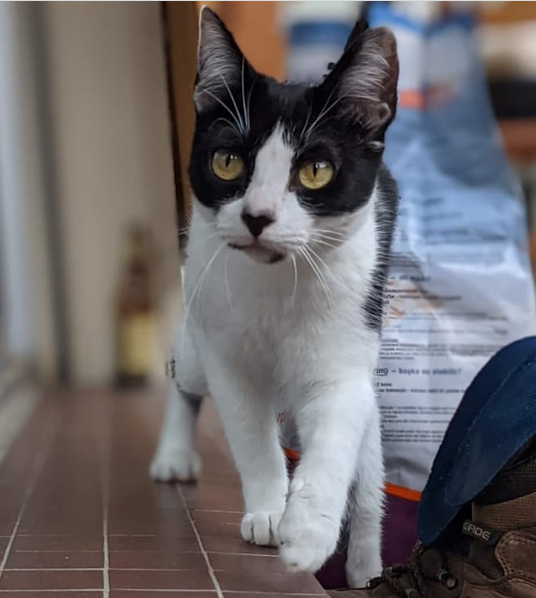
\includegraphics[height=40mm,width=35mm,clip]{Images/guinesse.png}};
			\node (rect) [draw=MPTgrey,fill=white, very thick,minimum width=1.5cm,minimum height=0.8cm,visible on=<2>] at(0,-0.6) {\scshape \textcolor{MPTgrey}{CHAT}};
			\node (insta)[]  at([yshift = -4]ref.south) {\raisebox{-1.5mm}{
\includegraphics[width = 4mm]{Images/insta.jpeg} \xspace}\footnotesize \href{https://www.instagram.com/guinesse_thecat/?hl=fr}{guinesse$\_$thecat}};
			\node (ref1) [right=of ref] {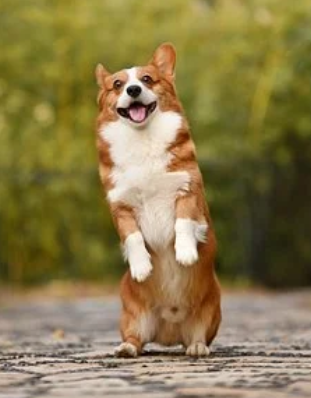
\includegraphics[height=40mm,width=35mm,clip]{Images/gorky.png}};
			\node (rect1) [draw=MPTgrey,fill=white, very thick,minimum width=2.5cm,minimum height=0.8cm,visible on=<2>] at(4.85,-0.6) {\scshape \textcolor{MPTgrey}{NON-CHAT}};
			\node (wiki)[]  at([yshift = -4]ref1.south) {\footnotesize  \href{https://fr.wikipedia.org/wiki/Welsh_Corgi_Pembroke}{Welsh Corgi Pembroke}};
		\end{tikzpicture}
		
}
\only<3>{
	\Large \textbf{Reconnaissance de chiffres manuscrits}\\[1.5em]
	
	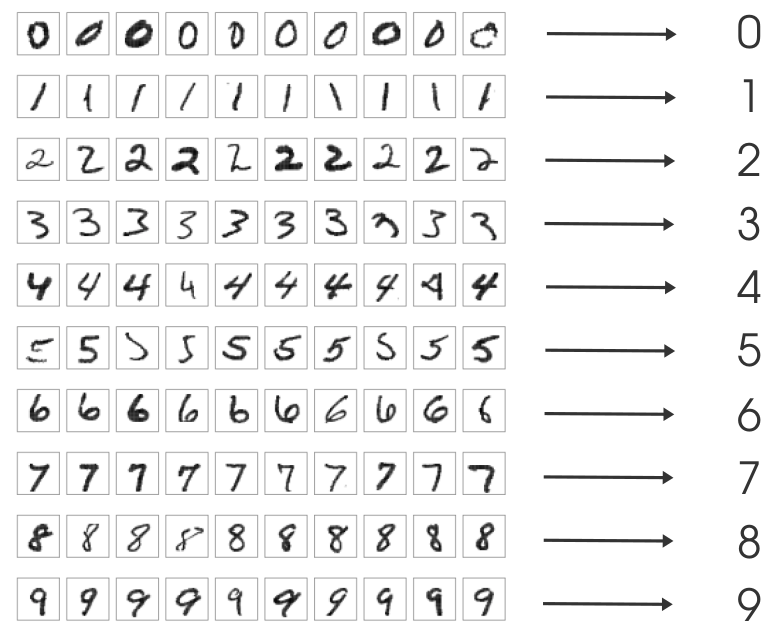
\includegraphics[height=0.55\textheight]{Images/nombres.png}
	
	\vspace*{0.3em}
	\footnotesize{\textcolor{MPTgrey}{Image tirée d'une présentation donnée par Chloé-Agathe\\ Azencott en 2019 aux Mines de Paris (Fontainebleau)} }
	}
%
\only<4>{
	\Large \textbf{Segmentation de marché}\\[0.4em]
	\normalsize Objectif : identifier des groupes d’usagers ou de clients dont le \\ comportement est similaire afin de mieux comprendre leur profil\\[0.8em]
		
	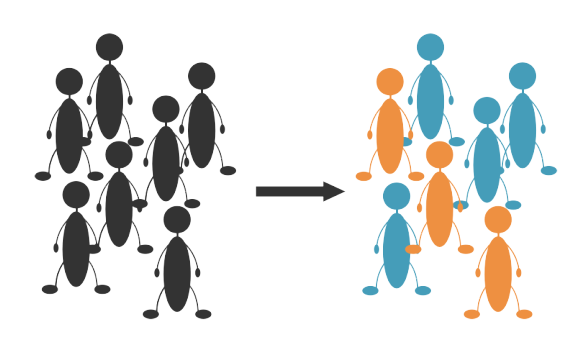
\includegraphics[height=0.5\textheight]{Images/segmentation.png}
	
		\vspace*{0.3em}
	\footnotesize{\textcolor{MPTgrey}{Image tirée d'une présentation donnée par Chloé-Agathe\\ Azencott en 2019 aux Mines de Paris (Fontainebleau)} }	
}
%
\only<5>{
	\Large \textbf{Prédiction de clics}\\[1.5em]

	
	
	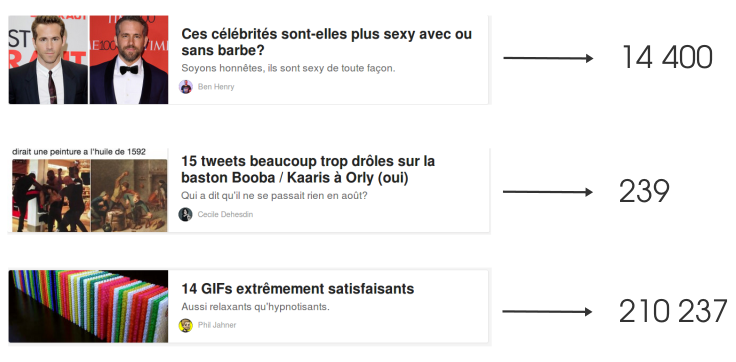
\includegraphics[height=0.5\textheight]{Images/clics.png}
	
	\vspace*{0.3em}
	\footnotesize{\textcolor{MPTgrey}{Image tirée d'une présentation donnée par Chloé-Agathe\\ Azencott en 2019 aux Mines de Paris (Fontainebleau)} }
	
}

\only<6>{
	\Large \textbf{Segmentation d'image}\\[1.5em]
	
	
	
	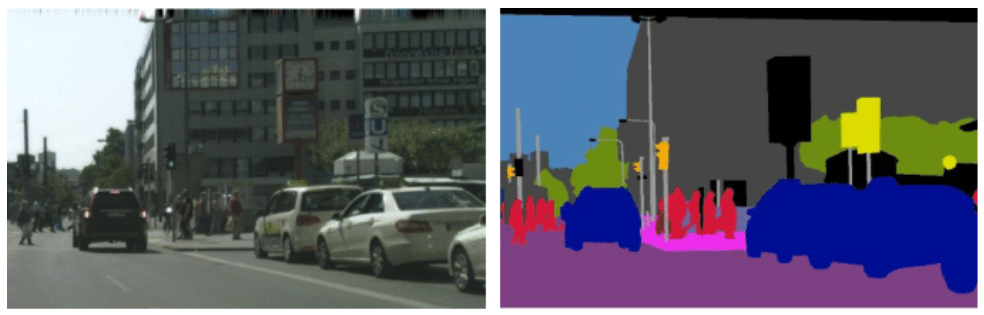
\includegraphics[width=0.98\textwidth]{Images/segmentationImage.png}
	
	\vspace*{0.3em}
	\footnotesize{\textcolor{MPTgrey}{Image tirée du site \textit{\href{https://larevueia.fr/quest-ce-que-la-segmentation-dimages/}{La revue IA}}} }
	
}

\only<7>{
	\Large \textbf{Compression d'image}\\[1.5em]
	
	
		\begin{tikzpicture}
	\node (ref) [] {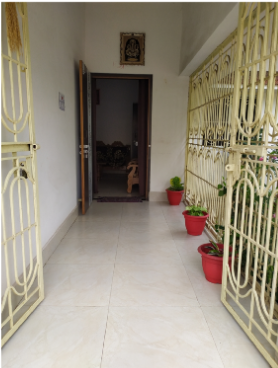
\includegraphics[height=40mm,width=35mm,clip]{Images/compr.png}};
	\node (note)[]  at([yshift = -4]ref.south) {\footnotesize Image originale};
	\node (ref1) [] at([xshift =60]ref.east) {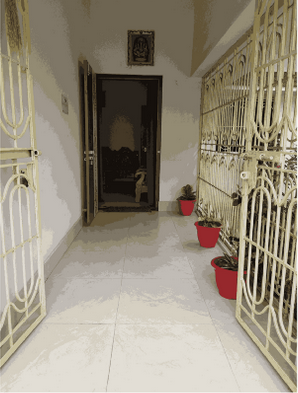
\includegraphics[height=40mm,width=35mm,clip]{Images/compr2.png}};
	\node (note1)[]  at([yshift = -4]ref1.south) {\footnotesize Image compressée (16 couleurs)};
		\node (ref2) at([xshift =60]ref1.east) {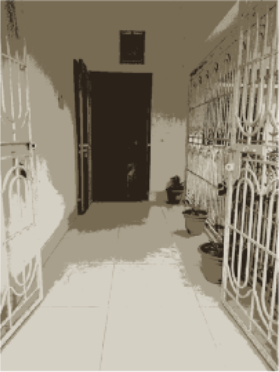
\includegraphics[height=40mm,width=35mm,clip]{Images/compr3.png}};
			\node (note2)[]  at([yshift = -4]ref2.south) {\footnotesize Image compressée (4 couleurs)};
\end{tikzpicture}
	
	\vspace*{0.3em}
	\footnotesize{\textcolor{MPTgrey}{Image tirée du site \href{https://towardsdatascience.com/image-compression-using-k-means-clustering-aa0c91bb0eeb}{Towards Data Science} }}
	
}
	\end{center}
	\note{D'après vous comme l'algo fait pour reconnaitre chien ou chat ? }
\end{frame}

%-------------------------------------------------------------------------------------------------------------------------------------------
\begin{frame}{Ingrédients et objectif de l'apprentissage}
	
	\vspace{-1em}
\begin{minipt}[1]{0.2}	
	
%	\begin{itemize}
%		\item \textbf{Les données}\\[1em]
%		\item \only<1>\textbf{L'algorithme d'apprentissage}} \only<2->{\bfblue{L'algorithme d'apprentissage}} : procédure qui, à partir des données, produit/fournit un modèle\\[0.5em]
%\end{itemize}

\only<1>{	\begin{itemize}
		\item \textbf{Les données}\\[1em]
		\item \textbf{L'algorithme d'apprentissage} : procédure qui, à partir des données, produit/fournit un modèle\\[0.5em]
	\end{itemize}}

\only<2->{	\begin{itemize}
	\item \textbf{Les données}\\[1em]
	\item \only<1>{\textbf{L'algorithme d'apprentissage}} \only<2->{\bfblue{L'algorithme d'apprentissage}} : procédure qui, à partir des données, produit/fournit un modèle\\[0.5em]
\end{itemize}
}
\end{minipt}

\textcolor{MPTgrey}{ex : chat ou non --- modèle qui estime si c'est une photo de chat ou non \\
\phantom{ex : } seg. de marché --- modèle qui retourne des groupes d'individus \\[2em]}


\uncover<3->{
\begin{minipc}[0.06]{0.15}
	%\begin{center}
		\warning
		%$\mathbf{\textcolor{MPTblue}{(1)}}$
	%\end{center}
	%\vspace*{-.25\baselineskip}
	%
\includegraphics[height = 0.08\textheight]{Back.pdf}
\end{minipc}
\begin{minipc}[0.93]{0.15}
\textit{garbage in, garbage out} : si les données ne sont pas pertinentes ou de mauvaises qualité le modèle produit ne sera pas satisfaisant. Il est important que le \textit{data scientist} prépare les données (supprimer les données aberrantes, gérer les données manquantes, sélectionner une représentation pertinente, etc)
\end{minipc}
}

\vspace*{2em}

\uncover<4->{

\bftitle{Objectif} \hsp Modéliser un phénomène à partir de données/d'exemples \\
\phantom{\bftitle{Objectif} \hsp}Le modèle est obtenu en \textbf{optimisant un certain critère}\\[1em]
}


\uncover<5->{ 
	\textcolor{MPTgrey}{ex : chat ou non --- minimiser les erreurs de classification  \\
		\phantom{ex :}  seg. de marché --- maximiser la proximité entre individus d'un même groupe
%		\phantom{ex :}   groupe \\[2em]
	}

}
	
\end{frame}

%------------------------------------------------------------------------------------------
%------------------------------------------------------------------------------------------

\begin{frame}{Pourquoi utiliser le machine learning ?}
	
	L'apprentissage automatique peut servir à résoudre des problèmes\\[2em]
	
	\begin{itemize}
		\item que l’on sait résoudre, mais dont on ne sait formaliser en termes algorithmiques comment nous les résolvons\\
		\textcolor{MPTgrey}{ex : reconnaissance d'images, compréhension du langage naturel}  \\[2em]
		\item que l’on ne sait pas résoudre car les données sont \eg complexe et volumineuses \\
		\textcolor{MPTgrey}{ex : données astrophysiques, données génomiques}  \\[2em]
		\item  que l’on sait résoudre, mais avec des procédures (déterministes) trop gourmandes en ressources informatiques\\
		\textcolor{MPTgrey}{ex : prédiction d’interactions entre molécules de grande taille pour lesquelles les simulations sont très lourdes}  \\[2em] 
	\end{itemize}
	
%\phantom{a} \hfill \footnotesize \textcolor{MPTgrey}{Texte tiré de l'ouvrage \textit{\href{http://cazencott.info/dotclear/public/lectures/IntroML_Azencott.pdf}{Introduction au Machine Learning}} de Chloé-Agathe Azencott}
\end{frame}


%------------------------------------------------------------------------------------------
%------------------------------------------------------------------------------------------

\begin{frame}{Types d'apprentissage}
	
Il existe deux principaux types d'apprentissage : \\[4em]
	
	\begin{center}
		
		\bfblue{1.} \hsp \textbf{L'apprentissage supervisé}\\[3em]
		\bfblue{2.} \hsp \textbf{L'apprentissage non supervisé}\\[4em]
		
		 \end{center}
	 		
		Cette liste n'est pas du tout exhaustive. L'apprentissage automatique est un champ assez vaste et d'autres types d'apprentissage existent comme \eg l'apprentissage semi-supervisé et l'apprentissage par renforcement
\end{frame}


%------------------------------------------------------------------------------------------
%------------------------------------------------------------------------------------------


\begin{frame}{Apprentissage supervisé - analogie}

\vspace*{-1em}
\begin{minipc}[1]{0.35}
	\begin{center}
		
\only<1>{	\large Algorithme classique\\
	\normalsize	\textcolor{MPTgrey}{ex : modèles météorologiques déterministes }}

\only<2>{\large \textcolor{MPTblue}{Algorithme d'apprentissage supervisé}\\
\phantom{ex : modèles météorologiques déterministes }}

	\end{center}
\end{minipc}	

\begin{minipt}[1]{0.69}	
		\begin{center}
			\begin{tikzpicture}
				
				
				\node (rect) [draw=MPTgrey,rounded corners=7pt, fill=white, very thick,minimum width=3cm,minimum height=1.5cm,visible on=<1->] {\large Ingrédients};
				%\draw [->] (rect.east) to (rect1.west);
				\node (rect1) at([xshift = 3cm]rect.east)  [draw=MPTgrey,rounded corners=7pt, fill=MPTgrey!30, very thick,minimum width=3cm,minimum height=1.5cm,visible on=<1->] {};
				\draw[line width = 1.6pt, MPTgrey, ->, >=Triangle, visible on = <1->] (rect.east) -- ([xshift = -0.1cm]rect1.west);
				\node (rect2) at([xshift = 3cm]rect1.east)  [draw=MPTgrey,rounded corners=7pt, fill=white, very thick,dashed, minimum width=3cm,minimum height=1.5cm,visible on=<1-2>] {\large {Gâteau}};	
				\node (rect2) at([xshift = 3cm]rect1.east)  [draw=MPTblue,rounded corners=7pt, fill=white, very thick,dashed, minimum width=3cm,minimum height=1.5cm,visible on=<2>] {\large \textcolor{MPTblue}{Recette}};
				\draw[line width = 1.6pt, MPTgrey, ->, >=Triangle, visible on = <1->] (rect1.east) -- ([xshift = -0.15cm]rect2.west);	
				\node (rect3) at([yshift = -2cm]rect1.south)  [draw=MPTgrey,rounded corners=7pt, fill=white, very thick, minimum width=3cm,minimum height=1.5cm,visible on=<1-2>] {\large {Recette}};	
				\node (rect3) at([yshift = -2cm]rect1.south)  [draw=MPTgrey,rounded corners=7pt, fill=white, very thick, minimum width=3cm,minimum height=1.5cm,visible on=<2>] {\large {Gâteau}};	
				\draw[line width = 1.6pt, MPTgrey, ->, >=Triangle, visible on = <1->] (rect3.north) -- ([yshift = -0.1cm]rect1.south);
	\end{tikzpicture}
\end{center}
\end{minipt}
	

\end{frame}

%------------------------------------------------------------------------------------------
%------------------------------------------------------------------------------------------

\begin{frame}{Apprentissage supervisé - Objectif}
	
\bftitle{Contexte} \hsp On observe des \textbf{données} $x_1,\dots,x_n$ pour $n$ individus ainsi que des\\
\phantom{\bftitle{Contexte} \hsp} \textbf{étiquettes} $y_1,\dots,y_n$ associées\\[0.1em]
\phantom{\bftitle{Contexte} \hsp} \textcolor{MPTgrey}{ex : $\color{MPTgrey} x_i$ = (âge, genre, diplôme) et $\color{MPTgrey} y_i$ = (salaire) de l'individu $\color{MPTgrey} i$}\\[1em]


\bftitle{Objectif} \hsp Apprendre un modèle à partir de $ (x_1,y_1), \dots, (x_n, y_n)$ qui prédit \\
\phantom{\bftitle{Objectif} \hsp}(au mieux) l'étiquette $y$ pour tout nouvel individu de donnée $x$\\[1.7em]
	
	
	\begin{minipt}[1]{0.69}	
		
			\only<1|handout:1>{	
				\begin{center}
					\begin{tikzpicture}
				
				
				\node (rect) [draw=MPTgrey,rounded corners=7pt, fill=white, very thick,minimum width=3cm,minimum height=1.5cm,visible on=<1>] {\large Observations};
				\node (text) at([yshift = -0.4cm]rect.south) [visible on=<1>] {\large $x_1,\dots,x_n$};
				%\draw [->] (rect.east) to (rect1.west);
				\node (rect1) at([xshift = 3cm]rect.east)  [draw=MPTgrey,rounded corners=7pt, fill=MPTgrey!30, very thick,minimum width=3cm,minimum height=1.5cm,text width=2.8cm,text centered, visible on=<1>] {\large Algorithme d'apprentissage};
				\draw[line width = 1.6pt, MPTgrey, ->, >=Triangle, visible on = <1>] (rect.east) -- ([xshift = -0.1cm]rect1.west);
				\node (rect2) at([xshift = 3cm]rect1.east)  [draw=MPTblue,rounded corners=7pt, fill=white, very thick,dashed, minimum width=3cm,minimum height=1.5cm,visible on=<1>,text width=2.5cm,text centered] {\large \textcolor{MPTblue}{Modèle prédictif}};	
				\node (text) at([yshift = -0.4cm]rect2.south) [visible on=<1>] {\large $f(x) \approx y $};
				\draw[line width = 1.6pt, MPTgrey, ->, >=Triangle, visible on = <1>] (rect1.east) -- ([xshift = -0.15cm]rect2.west);	
				\node (rect3) at([yshift = -1.7cm]rect1.south)  [draw=MPTgrey,rounded corners=7pt, fill=white, very thick, minimum width=3cm,minimum height=1.5cm,visible on=<1>] {\large {Étiquettes}};	
				\node (text) at([yshift = -0.4cm]rect3.south) [visible on=<1>] {\large $y_1,\dots,y_n$};
				\draw[line width = 1.6pt, MPTgrey, ->, >=Triangle, visible on = <1>] (rect3.north) -- ([yshift = -0.1cm]rect1.south);
			\end{tikzpicture}
				\end{center}
		}
			\only<2|handout:2>{ 
				
				\vspace*{3.3em}
				
				Dans la suite du cours on va s'intéresser à des méthodes classiques d'apprentissage supervisé}

	\end{minipt}
	
	
\end{frame}

%------------------------------------------------------------------------------------------
%------------------------------------------------------------------------------------------


\begin{frame}{Apprentissage supervisé -- Exemple}
	
	\begin{center}
		\vspace*{-1em}
			\Large \textbf{Identifier des spams}\\[1.3em]
			\begin{tikzpicture}
				\node (ref) [] {
\includegraphics[height=20mm,width=70mm,clip]{Images/spam.jpeg}};
				\node (rect) [draw=MPTgrey,fill=white, very thick,minimum width=1.5cm,minimum height=0.6cm,visible on=<1>] at([yshift = -0.5cm, xshift=2.4cm]ref) {\scshape \normalsize \textcolor{MPTgrey}{SPAM}};
				\node (ref1) at ([yshift = -1.8cm]ref.south) {
\includegraphics[height=20mm,width=70mm,clip]{Images/nonspam.jpeg}};
			\node (rect) [draw=MPTgrey,fill=white, very thick,minimum width=1.5cm,minimum height=0.6cm,visible on=<1>] at([yshift = -0.6cm, xshift=2.4cm]ref1) {\scshape \normalsize \textcolor{MPTgrey}{NON-SPAM}};
			\end{tikzpicture}
		\end{center}
		\end{frame}

%------------------------------------------------------------------------------------------
%------------------------------------------------------------------------------------------


\begin{frame}{Apprentissage non supervisé - Objectif}
	
	\bftitle{Contexte} \hsp On observe des \textbf{données} $x_1,\dots,x_n$ pour $n$ individus mais \textbf{sans} \\ \phantom{\bftitle{Contexte} \hsp}  \textbf{étiquettes} associées (on dit qu'elles sont non étiquetées)\\[1em]
	
	
	\bftitle{Objectif} \hsp Modéliser les observations $x_1,\dots,x_n$ pour mieux les comprendre\\[0.2em]
	\phantom{\bftitle{Objectif} \hsp}En pratique, on détermine une fonction sur $\{x_1,\dots, x_n\}$ qui vérifie\\
	\phantom{\bftitle{Objectif} \hsp}certaines propriétés \\[4em]
	
	
	\begin{minipt}[1]{0.69}	
	\renewcommand \logowidth{13pt} %pour la taille du logo lampe
		\begin{center}
			\begin{tikzpicture}
				
				
				\node (rect) [draw=MPTgrey,rounded corners=7pt, fill=white, very thick,minimum width=3cm,minimum height=1.5cm,visible on=<1->] {\large Observations};
				\node (text) at([yshift = -0.4cm]rect.south) [visible on=<1->] {\large $x_1,\dots,x_n$};
				%\draw [->] (rect.east) to (rect1.west);
				\node (rect1) at([xshift = 3cm]rect.east)  [draw=MPTgrey,rounded corners=7pt, fill=MPTgrey!30, very thick,minimum width=3cm,minimum height=1.5cm,text width=2.8cm,text centered, visible on=<1->] {\large Algorithme d'apprentissage};
				\draw[line width = 1.6pt, MPTgrey, ->, >=Triangle, visible on = <1->] (rect.east) -- ([xshift = -0.1cm]rect1.west);
				\node (rect2) at([xshift = 3cm]rect1.east)  [draw=MPTblue,rounded corners=7pt, fill=white, very thick,dashed, minimum width=3cm,minimum height=1.5cm,visible on=<1->,text width=3.1cm,text centered] {\raisebox{2mm}{\raisebox{-.8mm}{\bclampe \xspace} \large \textcolor{MPTblue}{Observations}}};	
				\draw[line width = 1.6pt, MPTgrey, ->, >=Triangle, visible on = <1->] (rect1.east) -- ([xshift = -0.15cm]rect2.west);	
			\end{tikzpicture}
		\end{center}
	\end{minipt}
	
	
\end{frame}

%------------------------------------------------------------------------------------------
%------------------------------------------------------------------------------------------

\begin{frame}{Apprentissage non supervisé - Types}
	

	
	\begin{center}
		\vspace*{1.5em}
		
			Les principaux problèmes traités en apprentissage non supervisé sont :\\[3em]
			

				\begin{minipt}[0.54]{1}
				\only<1|handout:0>{	\begin{itemize}
						\item[\ex] \hsp Le clustering ou partitionnement\\
						\hsp (= classification non supervisé)\\[3em]						
							\item[\ex] \hsp La réduction de dimension\\[3em]
							\item[\ex] \hsp L'estimation de densité \\[3em]						
					\end{itemize}
				}
							\only<2|handout:1>{	\begin{itemize}
						\item[\ex] \hsp \textbf{Le clustering ou partitionnement\\
					\hsp (= classification non supervisée)}\\[3em]						
						\item[\ex] \hsp La réduction de dimension\\[3em]
						\item[\ex] \hsp L'estimation de densité \\[3em]						
				\end{itemize}
			}
				\end{minipt}
			\end{center}
\end{frame}

%------------------------------------------------------------------------------------------
%------------------------------------------------------------------------------------------


\begin{frame}{Clustering -- Objectif}
	
	\bftitle{Contexte} \hsp On observe des \textbf{données} $x_1,\dots,x_n$ pour $n$ individus \\[1em]
	
	
	\bftitle{Objectif} \hsp Identifier des groupes dans les données\\[0.8em]
	\phantom{\bftitle{Objectif} \hsp} Permet d'extraire de l'information sur les données, de mieux\\ \phantom{\bftitle{Objectif} \hsp} comprendre leurs caractéristiques générales
	\\[2.2em]
	
	
	\begin{minipt}[1]{0.69}	
		\renewcommand \logowidth{13pt} %pour la taille du logo lampe
		\begin{center}
			\begin{tikzpicture}
				
				
				\node (rect) [draw=MPTgrey,rounded corners=7pt, fill=white, very thick,minimum width=3cm,minimum height=1.5cm,visible on=<1->] {\large Observations};
				\node (text) at([yshift = -0.7cm]rect.south) [visible on=<1->] {\large $x_1,\dots,x_n$};
				%\draw [->] (rect.east) to (rect1.west);
				\node (rect1) at([xshift = 2.8cm]rect.east)  [draw=MPTgrey,rounded corners=7pt, fill=MPTgrey!30, very thick,minimum width=3cm,minimum height=1.5cm,text width=2.8cm,text centered, visible on=<1->] {\large Algorithme d'apprentissage};
				\draw[line width = 1.6pt, MPTgrey, ->, >=Triangle, visible on = <1->] (rect.east) -- ([xshift = -0.1cm]rect1.west);
				\node (rect2) at([xshift = 2.8cm]rect1.east)  [draw=white,rounded corners=7pt, fill=white, very thick,dashed, minimum width=3cm,minimum height=1.5cm,visible on=<1->,text width=3.1cm,text centered] {};
				\node (cir1) at([xshift = -1.2cm, yshift=1cm]rect2)  [draw=MPTblue,circle, minimum size=1.3cm, fill=white, very thick,visible on=<1->,text width=0.5cm,text centered] {$\C_1$};
				\node (cir1) at([xshift = -0.8cm,yshift=-0.3cm]rect2)  [draw=MPTblue,circle, minimum size=0.8cm, fill=white, very thick,visible on=<1->,text width=0.5cm,text centered] {$\C_2$};
				\node (cir1) at([xshift = 0.6cm,yshift=0.2cm]rect2)  [draw=MPTblue,circle, minimum size=1.5cm, fill=white, very thick,visible on=<1->,text width=0.5cm,text centered] {$\C_K$};
				\node (cir1) at([xshift = 1.6cm,yshift=1.2cm]rect2)  [draw=MPTblue,circle, minimum size=0.6cm, fill=white, very thick,visible on=<1->,text width=0.5cm,text centered] {$\C_3$};
				\draw[line width = 1.6pt, MPTgrey, ->, >=Triangle, visible on = <1->] (rect1.east) -- ([xshift = -0.15cm]rect2.west);
				\node (text) at([yshift = -0.7cm]rect2.south) [visible on=<1->] {\large $\{x_1,\dots,x_n \}=\displaystyle \bigcup_{i=n}^K \C_k$};	
			\end{tikzpicture}
		\end{center}
	\end{minipt}
	
	
\end{frame}

%------------------------------------------------------------------------------------------
%------------------------------------------------------------------------------------------

\begin{frame}{Clustering -- Exemple}
	\begin{center}

	\Large \textbf{Identification de gènes similaires}\\[0.4em]
	\normalsize Permet de faire des hypothèses sur le rôle des gènes\\[1.5em]
	
	
	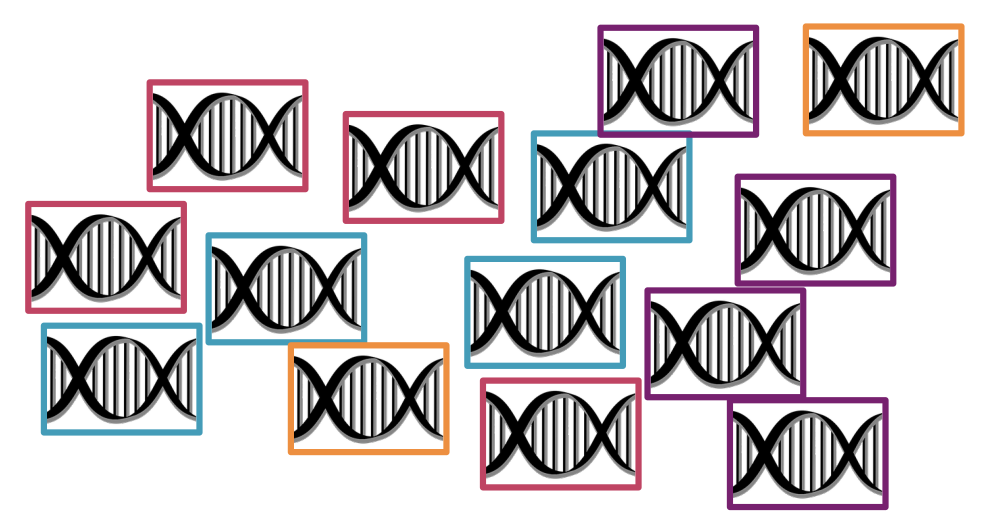
\includegraphics[height=0.5\textheight]{Images/genesGroupes.png}
	
	\vspace*{1em}
	\footnotesize{\textcolor{MPTgrey}{Image tirée d'une présentation donnée par Chloé-Agathe\\ Azencott en 2019 aux Mines de Paris (Fontainebleau)}\\[2.2em]}
		
\end{center}
\end{frame}

%------------------------------------------------------------------------------------------
%------------------------------------------------------------------------------------------

\begin{frame}{Réduction de dimension -- Objectif}
	
	\bftitle{Contexte} \hsp On observe des \textbf{données} $x_1,\dots,x_n$ pour $n$ individus \\[1em]
	
	
	\bftitle{Objectif} \hsp Trouver une représentation des données dans un espace de dimension\\ \phantom{\bftitle{Objectif} \hsp}plus faible que celui d'origine\\[0.8em]
	\phantom{\bftitle{Objectif} \hsp}Permet de réduire les temps de
	calcul et l’espace mémoire utilisé pour\\ \phantom{\bftitle{Objectif} \hsp}le stockage les données, de mieux visualiser les données, d’améliorer\\ \phantom{\bftitle{Objectif} \hsp}les performances d’un algorithme d’apprentissage supervisé entraîné\\ \phantom{\bftitle{Objectif} \hsp}ensuite sur ces données	\\[2.5em]
	
	
	\begin{minipt}[1]{0.69}	
		\renewcommand \logowidth{13pt} %pour la taille du logo lampe
		\begin{center}
			\begin{tikzpicture}
				
				
				\node (rect) [draw=MPTgrey,rounded corners=7pt, fill=white, very thick,minimum width=3cm,minimum height=1.5cm,visible on=<1->] {\large Observations};
				\node (text) at([yshift = -0.7cm]rect.south) [visible on=<1->] {\large $x_1,\dots,x_n$};
				%\draw [->] (rect.east) to (rect1.west);
				\node (rect1) at([xshift = 2.8cm]rect.east)  [draw=MPTgrey,rounded corners=7pt, fill=MPTgrey!30, very thick,minimum width=3cm,minimum height=1.5cm,text width=2.8cm,text centered, visible on=<1->] {\large Algorithme d'apprentissage};
				\draw[line width = 1.6pt, MPTgrey, ->, >=Triangle, visible on = <1->] (rect.east) -- ([xshift = -0.1cm]rect1.west);
				\node (rect2) at([xshift = 2.8cm]rect1.east)  [draw=MPTblue,rounded corners=7pt, fill=white, very thick,dashed, minimum width=2cm,minimum height=1cm,visible on=<1->,text width=2cm,text centered] {Observations réduites};
				\draw[line width = 1.6pt, MPTgrey, ->, >=Triangle, visible on = <1->] (rect1.east) -- ([xshift = -0.15cm]rect2.west);
				\node (text) at([yshift = -0.7cm]rect2.south) [visible on=<1->] {\large $z_1,\dots,z_n$};	
			\end{tikzpicture}
		\end{center}
	\end{minipt}
	
	
\end{frame}

%------------------------------------------------------------------------------------------
%------------------------------------------------------------------------------------------

\begin{frame}[fragile]{Réduction de dimension  -- Exemple}
	\begin{center}
		\vspace*{-1em}
		\Large \textbf{Visualisation de génomes en 2 dimensions}\\[0.4em]
		\normalsize Permet de visualiser la correspondance entre la structure des génomes et la position géographique des individus\\[1.5em]
		
		
		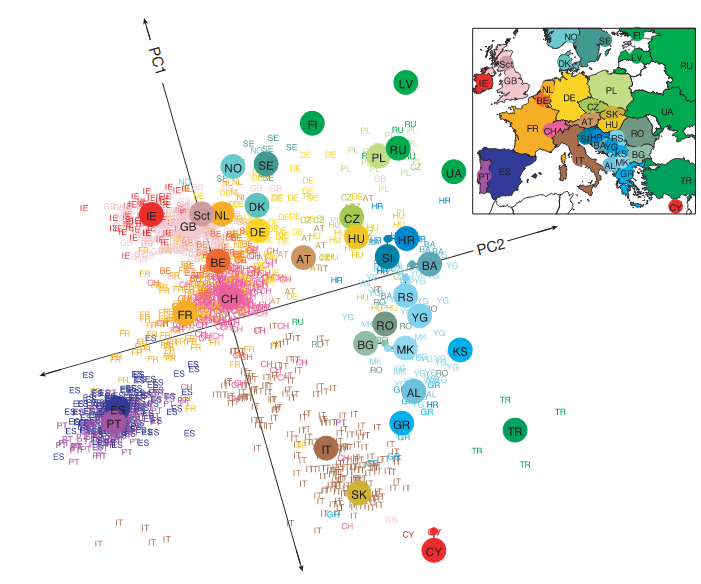
\includegraphics[height=0.58\textheight]{Images/adnEurope.png}
		
		\vspace*{0.5em}
	\footnotesize{\textcolor{MPTgrey}{Image tirée de l'article \href{https://www.nature.com/articles/nature07331}{November et al. (2008)}}}
		
	\end{center}
\end{frame}


%------------------------------------------------------------------------------------------
%------------------------------------------------------------------------------------------


\begin{frame}[fragile]{L'estimation de densité -- Objectif}
	\vspace*{2em}
	
		\bftitle{Contexte} \hsp On observe des \textbf{données} $x_1,\dots,x_n$ qu'on suppose être des\\ \phantom{\bftitle{Contexte} \hsp}réalisations (indépendantes) d'une variable aléatoire $X \sim \L$\\[1em]
	
	
	\bftitle{Objectif} \hsp Estimer $\L$ à partir des données $x_1,\dots,x_n$ \\[2.5em]
	
\begin{minipt}[1]{0.69}	
			\begin{tikzpicture}			

				
				\begin{axis}[school, width = 0.75\textwidth,  xlabel = $x$ , ylabel = , xmin = -8, xmax = 8.5, ymin = 0, ymax = 0.55, xtick = {-8,0,8},xticklabels={-8,0,8}, ytick=\empty, axis x line* = bottom, axis y line* = middle,  legend columns=3, legend style={draw = none, at={(0.5,-0.2)}, anchor=north}, width=5in, height=2in,visible on=<1>%, unit vector ratio* = {0.1 10}, scale = 1.25
					]

					\addplot[ybar,ybar interval=0, fill=cyan!20,visible on=<1>] coordinates { (-8.0,0.004) (-7.5,0) (-7.0,0) (-6.5,0) (-6.0,0) (-5.5,0) (-5.0,0.008) (-4.5,0.004) (-4.0,0.004) (-3.5,0.008) (-3.0,0.024) (-2.5,0.028) (-2.0,0.092) (-1.5,0.152) (-1.0,0.284) (-0.5,0.416)  (0.0,0.392)  (0.5,0.220)  (1.0, 0.132)  (1.5,0.132)  (2.0, 0.044)  (2.5,0.012)  (3.0, 0.008) (3.5,0.016)  (4.0,0.004)  (4.5,0.000)  (5.0,0.004)  (5.5,0.008)  (6.0,0.004)  (6.5,0.004)};

					
					\addplot[very thick, MPTblue, opacity=0.9,mark = none, domain = -8:9, samples = 200,visible on=<1>] {gauss(0,1)};
					\node[visible on=<1>] at(2.2,0.3){$\color{MPTblue} \L \,\, ?$};
					\node[visible on=<1>] at(-5,0.3){histogramme de $x_1,\dots, x_n$};
					
				\end{axis}
				
				%\begin{axis}[visible on=<4>]
				%\end{axis}
			\end{tikzpicture}
			%\tikzexternaldisable
			%}
		
	\end{minipt}
\end{frame}

%------------------------------------------------------------------------------------------
%------------------------------------------------------------------------------------------

\begin{frame}{Quizz}
	\vspace*{2em}
	
	\begin{center}
		\href{https://docs.google.com/forms/d/e/1FAIpQLSdqg3E4LdYxwYwDfNGjBbZ6Wg6-2cCIDo9tpXtvLKn94hXwtQ/viewform?usp=sf_link}{\textcolor{MPTblue}{\textbf{Est-ce de l'apprentissage supervisé ou non supervisé ?}}}\\[2em]
		
		\begin{minipt}[0.43]{1}
		
\includegraphics[height=0.5\textheight]{Images/frame.png}
				\end{minipt} 
			\begin{minipt}[0.32]{1} \hfill
				\vspace*{-11.8em}
				
			 Chat ou non ?\\[0.5em]
				 Reconnaissance de chiffres \\[0.5em]
				 Segmentation de marché\\[0.5em]
				Prédiction de clics\\[0.5em]
				 Segmentation d'image\\[0.5em]
				 Compression d'image				
		\end{minipt}
		
		
	\end{center}
	
\end{frame}

%------------------------------------------------------------------------------------------
%------------------------------------------------------------------------------------------

\begin{frame}{Modèles d'apprentissage}
	\begin{minipt}[1]{0.45}
		
	Voici quelques exemples d'approches, de modèles ou familles de modèles que vous verrez dans certains cours du master MIASHS :\\		
	\begin{itemize}
		\item \textit{Classification supervisée et non supervisée} (S1) : \\[0.7em]
		%Séance 1 \hsp --- \hsp Introduction \\[.2em]
		%Séance 2 \hsp --- \hsp 
		Régression logistique \hfill \only<2->{\textcolor{MPTgrey}{Supervisé}}\\[.2em]
		%Séance 3 \hsp --- \hsp 
		Arbres de décision (CART) \hfill \only<2->{\textcolor{MPTgrey}{Supervisé}}\\[.2em]
		%Séance 4 \hsp --- \hsp
		 Machine à noyaux et SVM \hfill\only<2->{\textcolor{MPTgrey}{Supervisé}}\\[.2em]
		%Séance 5 \hsp --- \hsp 
		Clustering \hfill\only<2->{\textcolor{MPTgrey}{Non supervisé}}		
	\end{itemize}
	\end{minipt}

	\begin{minipt}[1]{0.45}
			\only<3>{ 	\vspace*{2.5em}
				Dans la suite de cette séance, nous allons discuter plus en détails de l'apprentissage supervisé et introduire les \textbf{questions} et les \textbf{notions} que vous devrez avoir en tête lorsque vous serez face à un problème d'apprentissage supervisé ainsi que les \textbf{étapes essentielles} que vous mettrez en place pour résoudre ce problème}
		\only<1-2>{
	\begin{itemize}	
		\item \textit{Modèles de régression linéaire et outils du diagnostic} (S1) : régression linéaire\\[1em]
		\item \textit{Analyse de données multidimensionnelles} (S1) : réduction de dimension\\[1em]
		\item \textit{Régression logistique et poissonnienne} (S2) : régression logistique\\[1em]
		\item \textit{Apprentissage profond} (S2) et \textit{Analyse d’images} (S3) : deep learning\\[1em]
	%	\item Régularisation et optimisation
	\end{itemize}}
	\end{minipt}
\end{frame}

%------------------------------------------------------------------------------------------
%------------------------------------------------------------------------------------------

%------------------------------------------------------------------------------------------
%------------------------------------------------------------------------------------------

\section{L'apprentissage supervisé}

%------------------------------------------------------------------------------------------
%------------------------------------------------------------------------------------------

\subsection{Cadre de l'apprentissage supervisé}

%------------------------------------------------------------------------------------------
%------------------------------------------------------------------------------------------

\begin{frame}{Objectif}
	
	\bftitle{Contexte} \hsp On observe une donnée $x \in \X$ et on souhaite prédire son label\\ \phantom{\bftitle{Contexte} \hsp}associé $y \in \Y$ qui n'a pas été observé\\
	\phantom{\bftitle{Contexte} \hsp}\textcolor{MPTgrey}{ex : $\color{MPTgrey} x$ = (âge, genre, diplôme) et $\color{MPTgrey} y$ = (salaire) pour un individu}\\[2em]
	
	\begin{itemize}
		\item \hsp $x$ \,  : \, donnée observée, donnée d’entrée, variables explicatives\\[0.2em]
		\item \hsp  $y$ \, : \, label, étiquette, cible, variable à expliquer, variable réponse\\[3em]
	\end{itemize}

\bftitle{Objectif} \hsp Trouver un \textbf{modèle}/ une \textbf{règle de décision}, c'est-à-dire une\\ \phantom{\bftitle{Objectif} \hsp}fonction (mesurable) $f : \X \to \Y$, telle que $f(x)$ soit le plus\\ \phantom{\bftitle{Objectif} \hsp}proche possible de $y$\\[2em]

\bftitle{Remarque} \hsp  On va voir par la suite qu'une règle de décision $f$ dépend\\ \phantom{\bftitle{Remarque} \hsp}(entre autres) du type de problème d’apprentissage supervisé\\ \phantom{\bftitle{Remarque} \hsp}considéré, \ie de la nature de $\Y$\\[2em]
\end{frame}

%------------------------------------------------------------------------------------------
%------------------------------------------------------------------------------------------

\begin{frame}{Types d'apprentissage supervisé}
	
	Il existe différents types de problèmes en apprentissage supervisé suivant la nature de $\Y$, l'espace des labels\\[1.5em]
 \begin{itemize}
 	\item $\Y  \subset \bbR$ non fini : \bfblue{problème de régression}\\[2em]
 	%Le label $y$ (vu comme une variable) est une variable \textbf{quantitative}
 	% \\[2em]
 	 	\item $\text{Card}\left(\Y\right)=2$ : \bfblue{problème de classification bivariée/binaire}\\[0.1em]
 	 	Quel que soit $\Y$, on se ramène souvent aux cas $\Y=\{0,1\}$ ou $\Y=\{-1,1\}$ \\[2em]
 	 	%La variable $y$ est dite \textbf{qualitative} \\[2em]
 %	La variable $y$ est dite \textbf{qualitative} et, quelle que soit la nature de $\Y$, on se ramène souvent aux cas $\Y=\{0,1\}$ ou $\Y=\{-1,1\}$
\item $\text{Card}\left(\Y\right)= C >2$ : \bfblue{problème de classification multi-classe}\\[0.1em]
 	 	 	Quel que soit $\Y$, on se ramène souvent au cas $\Y=\{1,\dots,C\}$  \\[2em]
 %	La variable $y$ est dite \textbf{qualitative}


 \end{itemize}
\end{frame}

%------------------------------------------------------------------------------------------
%------------------------------------------------------------------------------------------

\begin{frame}{Types d'apprentissage supervisé -- Quizz}
	
\begin{center}
\large \textbf{	Régression ou classification ?}\\[1em]
\normalsize
	\begin{minipt}[01]{0.65} \hfill
	
	Identifier en quelle langue un texte est écrit \\
	\only<2->{\textcolor{MPTgrey}{Classification multi-classe}}\\[0.5em]
	%
	Identifier si une transaction financière est frauduleuse ou non \\
	\only<3->{\textcolor{MPTgrey}{Classification binaire}}\\[0.5em]
	%
	Prédire la probabilité de développer une maladie \\
	\only<4->{\textcolor{MPTgrey}{Régression}}\\[0.5em]
	%
	Prédire l'espèce d'une plante donnée\\
	\only<5->{\textcolor{MPTgrey}{Classification multi-classe}}\\[0.5em]
	%
	Prédire le prix d’une action en bourse\\
	\only<6->{\textcolor{MPTgrey}{Régression}}\\[0.5em]
	%
	Prédire le nombre de clics sur un lien\\	
\only<7->{\textcolor{MPTgrey}{Régression}}\\[0.5em]		
\end{minipt}
\end{center}
\end{frame}

%------------------------------------------------------------------------------------------
%------------------------------------------------------------------------------------------
%------------------------------------------------------------------------------------------
%------------------------------------------------------------------------------------------
\begin{frame}{Les KNN : exemple introductif}
	\bftitle{Objectif} \hsp On observe des {données} $x_1,\dots,x_n \in \X$ ainsi que des {étiquettes}\\
	\phantom{\bftitle{Objectif} \hsp}$y_1,\dots,y_n \in \Y $ et l'on souhaite estimer l'étiquette d'une nouvelle\\\phantom{\bftitle{Objectif} \hsp} observation $x \in \X$\\[2em]
	%= \{1,\dots, K\}
	
	\begin{minipc}[0.06]{0.15}
		\raisebox{1.5mm}{\bclampe \xspace} 
	\end{minipc}
	\begin{minipc}[0.93]{0.15}
		\textit{Qui se ressemble s’assemble} : On étiquette $x$ en fonction des étiquettes $y_i$ des $K$ points $x_i$ du jeu de données dont il est le plus proche
	\end{minipc}
	
	\vspace{1em}
	\uncover<2->{
		\begin{itemize}
			\item $\N_K(x)$  : ensemble des $K$ plus proches voisin de $x$ parmi $x_1,\dots, x_n$
		\end{itemize}
		%}
	\vspace*{1.5em}
	
	\textcolor{MPTblue}{\large\textbf{Algorithme des $ \color{MPTblue} \mathbf{K}$ plus proches voisins (KNN)}}\hfill \textcolor{MPTgrey}{Classification}\\
	\vspace*{-0.25em}
	\begin{vblock}{}
		\begin{itemize}
			\item $\Y = \{1,\dots, C\}$ (problème de classification)\\[0.5em]
		\end{itemize}
		\pause
		\uncover<2->{	\,  $x$ prend l’étiquette majoritaire parmi celles de ses $K$ plus proches voisins (KNN) :
			$$ f_{\text{KNN}}(x) = \text{arg}\,\max\limits_{k \in \Y}\, \sum_{i  : x_i \in \N_K(x) } \mathbb{1}\left\{y_i = k\right\}$$
		}
		\vspace{-1em}
	\end{vblock}
	%	\hspace*{0.1em} \ex \, $f^*_{\text{KNN}}(x)$ est une estimation du classifieur de Bayes $$f^* : x \mapsto \text{arg}\,\max\limits_{k \in \Y}\, \mathbb{P}\left[Y=k \vert X=x\right]$$
	\vspace*{1em}
}
\end{frame}
%------------------------------------------------------------------------------------------
%------------------------------------------------------------------------------------------
\begin{frame}{Les KNN : exemple introductif}
	\vspace*{-2em}
\begin{center}
	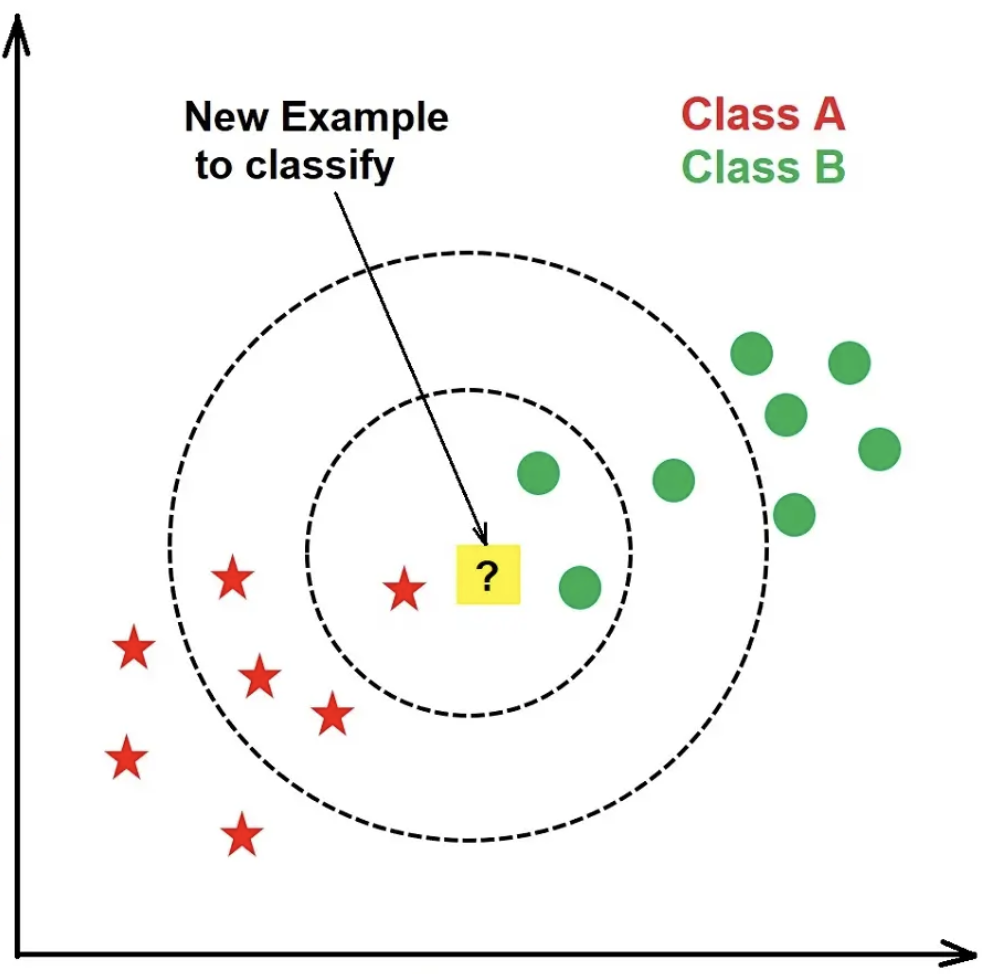
\includegraphics[height=0.6\textheight]{Images/knn.png}
	
	\vspace*{0.5em}
	\footnotesize{\textcolor{MPTgrey}{Image tirée du site \href{https://www.ejable.com/tech-corner/ai-machine-learning-and-deep-learning/k-nearest-neighbors/}{Ejable}}}
	
\end{center}
\vspace*{1em}

\begin{itemize}
\item $K=3$ : \uncover<2>{Classe B prédite}
\item $K=7$ : \uncover<2>{Classe A prédite}
\end{itemize}


\end{frame}

%------------------------------------------------------------------------------------------

\begin{frame}{Les KNN : exemple introductif}

%	\vspace{-1.5em}	
\textcolor{MPTblue}{\large\textbf{Algorithme des $ \color{MPTblue} \mathbf{K}$ plus proches voisins (KNN)} } \hfill \textcolor{MPTgrey}{Régression}\\
\vspace*{-0.25em}
\begin{vblock}{}
	\begin{itemize}
		\item $\Y = \bbR$ (problème de régression)\\[0.5em]
	\end{itemize}
	\uncover<2>{
		\, $x$ prend comme étiquette la moyenne de celles de ses K plus
		proches voisins : 
		%	\vspace*{-0.3em}
		$$ f_{\text{KNN}}(x) = \dfrac{1}{K} \sum_{i  : x_i \in \N_K(x) } y_i$$
	}
	\vspace{-1em}		
\end{vblock}
%\hspace*{0.1em} \ex \, $f^*_{\text{KNN}}(x)$ est une estimation de la règle $ f^* : x \mapsto  \mathbb{E}\left[Y \vert %X=x\right] $ qui minimise\\\phantom{\hspace*{0.1em} \ex \,}$R(f)$ pour la fonction de coût quadratique	\\[2.3em]	

\vspace*{1.5em}

\bftitle{Hyperparamètres du modèle :} \\[0.7em]

%\vspace*{-0.3em}
%\begin{vblock}{}
\begin{itemize}
	\item La \textbf{distance} entre deux points $x$ et $x'$ (permet de déterminer $\N_K(x)$) : elle est généralement choisie en fonction du type de données. Souvent on considère la distance euclidienne\\[0.5em]
	
	\item Le \textbf{nombre de voisins} $\mathbf{K}$ considérés : il est choisi par \textit{validation croisée}
\end{itemize}
\vspace{2em}

%	\vspace{1em}	
%\bftitle{Remarque} \hsp L'algorithme des $K$ plus proches voisins est une méthode simple à implémenter, non-paramétrique (pas d'hypothèses particulières sur le modèle) et s'adapte à tous types de données. Cependant 

\end{frame}

%------------------------------------------------------------------------------------------
%------------------------------------------------------------------------------------------

\begin{frame}{Qualités et défauts}
	
	L'algorithme des $K$ plus proches voisins : \\[2.3em]
	\begin{itemize}
		\item[\smiley] simple à implémenter\\[1em]
		\item[\smiley] méthode non-paramétrique : pas d'hypothèses particulières sur le modèle\\[1em]
		\item[\smiley] s'adapte à tous types de données\\[2em]
		\item[\frownie] intensif en temps de calcul : il faut calculer $n$ distances (compléxité de l’ordre de $O(nd)$ avec dim($\X)= d$) puis trouver les $K$ plus petites de ces distances (compléxité de l’ordre de $O(n \log K)$)\\[1em]
		\item[\frownie] susceptible de ne pas marcher en grande dimension, \ie quand $d$ est grand (fléau de la dimension) \textcolor{MPTgrey}{--- \textit{Pourquoi ?}}\\[3em]
	\end{itemize}
	
	
	
	
	
\end{frame}
%------------------------------------------------------------------------------------------
%------------------------------------------------------------------------------------------

\begin{frame}
	\begin{center}
		Faire le TP1 : \textit{La main à la pâte avec les KNN}
	\end{center}
	
	\vspace*{3em}
	\pause
	Remarques suite au TP :\\[1.5em]
	\begin{itemize}
		\item Besoin d'évaluer les performances des différents modèles possibles\\[1em]
		\item Besoin d'évaluer les performances du modèle sur des données desquelles la règle de décision de dépend pas
	\end{itemize}
	
		\vspace*{3em}
		
		\pause
		\begin{vblock}{}\centering
				Nous allons maintenant formaliser un peu mieux la problématique de l'apprentissage supervisé et introduire les principaux concepts
			\end{vblock}
\end{frame}
%------------------------------------------------------------------------------------------
%------------------------------------------------------------------------------------------
%------------------------------------------------------------------------------------------
%------------------------------------------------------------------------------------------

\subsubsection{ Formulation formelle de la problématique }

%------------------------------------------------------------------------------------------
%------------------------------------------------------------------------------------------

	\renewcommand \logowidth{19pt} % permet de changer la taille du logo ampoule
\begin{frame}{Problématique - point de vue probabiliste}

\bftitle{Objectif} \hsp Trouver une \textbf{règle de décision} $f : \X \to \Y$ (mesurable) telle que $f(x)$ soit le plus proche  possible de $y$ \only<2->{\bfred{pour n'importe} \bfred{quel} $\color{MPTred} \mathbf{x \in \X}$}\\
%\vspace*{0.5em}
	\uncover<3->{
	\begin{minipc}[0.06]{0.15}
		%\begin{center}
\raisebox{1.5mm}{\bclampe \xspace} 
	\end{minipc}
	\begin{minipc}[0.93]{0.15}
Puisqu'on ne veut pas fixer un $x$ en particulier 
%(on voudrait trouver une règle de décision qui fonctionne dans n'importe quel cas)
, on modélise la variable $x$ par un vecteur aléatoire $X$
	\end{minipc}
}

	\uncover<4->{
	\begin{minipc}[0.06]{0.15}
	\warning
\end{minipc}
\begin{minipc}[0.93]{0.15}
	Pour $(x_1,y_1), (x_2,y_2) \in \X \times \Y$ tels que $x_1=x_2$, on peut observer $y_1 \neq y_2$\\
	\textcolor{MPTgrey}{ex : erreurs lors de l'acquisition des données, manque d'informations, phénomène étudié de nature aléatoire}
\end{minipc}
}

	\uncover<5->{
	\begin{minipc}[0.06]{0.15}
	\raisebox{1.5mm}{\bclampe \xspace} 

\end{minipc}
\begin{minipc}[0.93]{0.15}
	Sachant $X$, on modélise la variable $y$ par une variable aléatoire $Y$
\end{minipc}

\bftitle{Notation} \hsp La loi de probabilité jointe de $(X,Y)$ est notée $\mathbb{P}_{X,Y}$\\[1.5em]
}

	\uncover<6->{
	\bftitle{Objectif} \hsp Trouver \, $f : \X \to \Y$ (mesurable) telle que la distance entre $Y$ et $f(X)$\\\phantom{\bftitle{Objectif} \hsp}soit la plus petite possible\\[1em]
}

	\uncover<7->{\bftitle{Question} \hsp Comment mesurer la distance entre $Y$ et $f(X)$ ?
	}
	

\end{frame}

%------------------------------------------------------------------------------------------
%------------------------------------------------------------------------------------------

\begin{frame}{Fonction de coût}
	
	\bftitle{Question} \hsp Comment mesurer la distance entre $Y$ et $f(X)$ ?\\[1em]
	
	\textcolor{MPTblue}{\large\textbf{Définition}}	
	\begin{vblock}{}
		Une fonction $\ell : \Y \times \Y \to \bbR_+$ est une \textbf{fonction de coût} si :\vspace{0.5em}
		\begin{itemize}
			\item  $\forall y \in \Y$ \hsp $\ell(y,y) = 0$\\
			\item  $\forall y, y' \in \Y, y\neq y'$ \hsp  $\ell(y,y') > 0$
		\end{itemize}
	\end{vblock}
	En pratique, on choisit $\ell$ telle que, pour tout $(x,y) \in \X \times \Y$, $\ell\left(y,f(x)\right)$ est d’autant plus grande que $f(x)$ est éloignée du (vrai) label $y$ : $\ell$ permet alors de quantifier la qualité d'une prédiction\\[1.5em]
	
\bftitle{Exemple} \hsp $\forall y, y' \in \Y$ \hsp $\ell(y,y') = \vert y-y'\vert$
\\ [0.3em]
\phantom{\bftitle{Exemple} \hsp $\forall y, y' \in \Y$ \hsp}$\ell(y,y') = \left(y-y'\right)^2$
\\[0.3em]
\phantom{\bftitle{Exemple} \hsp $\forall y, y' \in \Y$ \hsp}$\ell(y,y') = \mathbb{1}\left\{y \neq y' \right\}$
\\[0.5em]

	\uncover<2->{
	\begin{minipc}[0.06]{0.15}
		\warning
	\end{minipc}
	\begin{minipc}[0.93]{0.15}
	$\ell\left(Y,f(X)\right)$ est une variable aléatoire qui ne fournit pas une évaluation numérique de la distance entre $Y$ et $f(X)$ : on s'intéresse plutôt à son espérance
	\end{minipc}
}
%demander pour quel type de problèmes
%demander pourquoi indicatrice pas pour fonction continue

\end{frame}

%------------------------------------------------------------------------------------------
%------------------------------------------------------------------------------------------

\begin{frame}{Risque}
	\vspace*{-0.7em}
	\textcolor{MPTblue}{\large\textbf{Définition}}	
\begin{vblock}{}
	Le risque $R$ associé à une règle de décision $f$ et une fonction de risque $\ell$ est donnée par :\vspace{0.5em}
$$ R(f,\ell) = R(f) := \mathbb{E}_{\mathbb{P}_{X,Y}} \left[\ell\left(Y,f(X)\right)\right]$$
\vspace{-1.3em}
\end{vblock}
Un risque $R(f)$ fournit l'erreur moyenne de prévision que commet $f$ sur l'ensemble des valeurs possibles $x \in \X$ : il peut être vu comme une distance entre $f(X)$ et $Y$.\\[1.5em]

	\uncover<2->{
	\bftitle{Objectif} \hsp Trouver $f : \X \to \Y$ (mesurable) telle que la distance entre $Y$ et $f(X)$ \\\phantom{\bftitle{Objectif} \hsp}soit la plus petite possible. \\[1em]
	
	\uncover<3->{
	\phantom{\bftitle{Objectif} \hsp}La règle de décision optimale, notée $\boldsymbol{f^*}$ est donnée par :  
		$$ \boldsymbol{f^*= \text{\textbf{arg}}\,\min\limits_{f \in \F}\, R(f) = \text{\textbf{arg}}\,\min\limits_{f \in \F}\,\mathbb{E}_{\mathbb{P}_{X,Y}} \left[\ell\left(Y,f(X)\right)\right] }$$
	\phantom{\bftitle{Objectif} \hsp}$\F$ : ensemble des fonctions $f : \X \to \Y$ mesurables\\[0.5em]
}
}
	\uncover<4->{
	\begin{minipc}[0.06]{0.15}
		\warning
	\end{minipc}
	\begin{minipc}[0.93]{0.15}
		Cette règle de décision optimale dépend de la \textbf{loi} $\boldsymbol{\mathbb{P}_{X,Y}}$ \textbf{qui est inconnue}.
		Explicitons quand même cette fonction pour quelques fonctions de coût $\ell$ usuelles
	\end{minipc}
}
\note{quelles fonction de coût vous semble plus adapter à quels problèmes ?}
\end{frame}

%------------------------------------------------------------------------------------------
%------------------------------------------------------------------------------------------


\begin{frame}{Coût quadratique}
\bftitle{Question} \hsp Soit la fonction de coût $\ell : (y,y') \in \Y\times\Y \mapsto (y-y')^2 \in \bbR_+$\\\phantom{\bftitle{Question} \hsp}En supposant que nous avons accès à $\mathbb{P}_{X,Y}$, quelle est la règle\\\phantom{\bftitle{Question} \hsp}de décision $f^*$ optimale, \ie que vaut
$$ f^*= \text{arg}\,\min\limits_{f \in \F}\, R(f) \, \, ? $$ 

Supposons que $\mathbb{P}_{X,Y}$ admet une densité et que $\mathbb{E}\left[Y^2\right] < +\infty$ et $\mathbb{E}\left[\left(f(X)\right)^2\right] < +\infty$\\ [0.5em] On a :
\pause
$$
\begin{array}{lll}
	 R(f) &= &\mathbb{E}_{{X,Y}} \left[\left(Y-f(X)\right)^2\right]\\
	 & = &\mathbb{E}_{X} \left[\mathbb{E}_{Y|X} \left[\left(Y-f(X)\right)^2 \vert X\right]\right] \\[0.3em]
	 & = & \displaystyle \int_{\X} f_X(x) \int_{\Y} \left(y-f(x)\right)^2 \, f_{Y\vert X} (y\vert x) \, dy\ dx\\[1.5em]	 
\end{array}
$$

Pour minimiser $R(f)$, il suffit donc de minimiser, pour tout $x \in \X$, $$ g_x : t\in \Y \mapsto t^2 -2t \displaystyle \int_{\Y} y f_{Y\vert X} (y\vert x) \, dy$$ 

	 
\end{frame}

%------------------------------------------------------------------------------------------
%------------------------------------------------------------------------------------------


\begin{frame}{Coût quadratique}
Notons $g_x'$ et $g_x''$ les dérivées première et seconde de $g_x$ respectivement.\\[1em]
$$ g_x'(t) = 0  \hsp \Leftrightarrow \hsp t= \displaystyle \int_{\Y} y f_{Y\vert X} (y\vert x) \, dy = \mathbb{E} \left[Y \vert X=x\right] $$

et

$$g_x''(t) = 2 > 0$$

donc  $t=\mathbb{E} \left[Y \vert X=x\right] $ est un minimum global de $g_x$\\[2em]

		\textcolor{MPTred}{\large\textbf{Propriété}}
	\vspace*{-0.2em}	
	\begin{valblock}{}
		La règle de décision optimale $f^*$ qui minimise $R(f) = \mathbb{E}_{\mathbb{P}_{X,Y}} \left[\left(Y-f(X)\right)^2\right]$ est donnée, pour tout $x \in \X$, par 		
		$$ f^*(x) = \mathbb{E}\left[Y \vert X=x\right] $$	
		\vspace{-1.3em}	
	\end{valblock}
	
\end{frame}

%------------------------------------------------------------------------------------------
%------------------------------------------------------------------------------------------

\begin{frame}{Coût absolu et coût 0/1}
%	\bftitle{Question} \hsp Soit la fonction de coût $\ell : (y,y') \in \Y\times\Y \mapsto \vert y-y'\vert \in \bbR_+$\\\phantom{\bftitle{Question} \hsp}En supposant que nous avons accès à $\mathbb{P}_{X,Y}$, quelle est la règle\\\phantom{\bftitle{Question} \hsp}de décision optimale $f^*$ ?\\[4em]
	
	\textcolor{MPTblue}{\large\textbf{Coût absolu}}\hfill$\color{MPTgrey}\ell : (y,y') \in \Y\times\Y \mapsto \vert y-y'\vert \in \bbR_+$\\
	\vspace*{-0.2em}
	\begin{valblock}{}
		La règle de décision optimale $f^*$ qui minimise $R(f) = \mathbb{E}_{\mathbb{P}_{X,Y}} \left[ \vert Y - f(X) \vert \right]$ est donnée, pour tout $x \in \X$, par 		
		$$ f^*(x) = \text{médiane}\left(Y \vert X=x\right) $$	
		\vspace{-1.5em}	
	\end{valblock}
	
\vspace*{1em}
	
		\textcolor{MPTblue}{\large\textbf{Coût 0/1}}\hfill$\color{MPTgrey}\ell : (y,y') \in \Y\times\Y \mapsto \mathbb{1}\left\{y \neq y' \right\} \in \{0,1\}$\\
		\vspace*{-0.2em}
\begin{valblock}{}
	La règle de décision optimale $f^*$ qui minimise $R(f) = \mathbb{E}_{\mathbb{P}_{X,Y}} \left[ \mathbb{1}\left[Y \neq f(X) \right]\right]$ est donnée, pour tout $x \in \X$, par 		
	$$ f^*(x) = \text{arg}\,\max\limits_{k \in \Y}\, \mathbb{P}\left[Y=k \vert X=x\right]$$	
	
	Elle est connue sous le nom de \textbf{classifieur de Bayes }	
	
\end{valblock}
\note{Dire qu'on verra au 2nd semestre pour le coût 0/1}
\end{frame}

%------------------------------------------------------------------------------------------
%------------------------------------------------------------------------------------------

%\begin{frame}{Coût 0/1}
%	\bftitle{Question} \hsp Soit la fonction de coût $\ell : (y,y') \in \Y\times\Y \mapsto \mathbb{1}\left\{y \neq y' \right\} \in \{0,1\}$\\\phantom{\bftitle{Question} \hsp}En supposant que nous avons accès à $\mathbb{P}_{X,Y}$, quelle est la règle\\\phantom{\bftitle{Question} \hsp}de décision optimale $f^*$ ?\\[1.2em]
%Supposons que $\Y = \{1,\dots,C\}$, $C \geq 2$, \ie on regarde un problème de classification binaire (si $C=2$) ou de classification multi-classe ($C>2$)\\ [0.3em]	
%	On a :
%	$$
%	\begin{array}{lll}
%		R(f) &=& \mathbb{E}_{X} \left[\mathbb{E}_{Y|X} \left[\mathbb{1}\left\{Y \neq f(X) \right\} \vert X\right]\right] \\[0.3em]
%		& = & \displaystyle \int_{\X} f_X(x) \sum_{k=1}^C \mathbb{1}\left\{k \neq  f(x) \right\} \ \mathbb{P}\left[Y=k \vert X=x\right]\, dx\\[1em]	 
%	\end{array}
%	$$
%	\vspace*{1em}
%	
%	Pour minimiser $R(f)$, il suffit donc de minimiser, pour tout $x \in \X$, $$ g_x : t\in \Y \mapsto \sum_{k=1}^C \mathbb{1}\left\{k \neq  t \right\} \ \mathbb{P}\left[Y=k \vert X=x\right] =  1 - \mathbb{P}\left[Y=t \vert X=x\right] $$ 	
%\ie prendre $t = \text{arg}\,\max\limits_{k \in \Y}\, \mathbb{P}\left[Y=k \vert X=x\right]$
%
%\end{frame}

%------------------------------------------------------------------------------------------
%------------------------------------------------------------------------------------------

\begin{frame}
	
	\begin{center}
			\uncover<1->{
			\begin{minipc}[0.06]{0.1}
				\warning
			\end{minipc}
			\begin{minipc}[0.93]{0.1}
				La loi $\mathbb{P}_{X,Y}$ est inconnue : quelque soit la fonction de coût utilisée, nous n'avons pas accès à la règle de décision optimale $f^*$
			\end{minipc}
		}
		
		\vspace{5em}
		\uncover<2>{
			\begin{minipc}[0.06]{0.15}
				\raisebox{1.5mm}{\bclampe \xspace} 
			\end{minipc}
			\begin{minipc}[0.93]{0.15}
				On va utiliser les données observées $(x_1,y_1), \dots, (x_n, y_n) \in \X\times\Y$
			\end{minipc}
		}
	\end{center}
	\note{pour f optimal, remarquer que le classifieur du KNN est un estimateur de ces f}
\end{frame}
%------------------------------------------------------------------------------------------
%------------------------------------------------------------------------------------------

%\begin{frame}{Coût 0/1}
%
%	
%\textcolor{MPTred}{\large\textbf{Propriété}}
%\vspace*{-0.2em}	
%\begin{valblock}{}
%	La règle de décision optimale $f^*$ qui minimise $R(f) = \mathbb{E}_{\mathbb{P}_{X,Y}} \left[ \mathbb{1}\left[Y \neq f(X) \right]\right]$ est donnée, pour tout $x \in \X$, par 		
%	$$ f^*(x) = \text{arg}\,\max\limits_{k \in \Y}\, \mathbb{P}\left[Y=k \vert X=x\right]$$	
%	
%	Elle est connue sous le nom de \textbf{classifieur de Bayes }	
%
%\end{valblock}
%
%	
%\bftitle{Remarque} \hsp Quand $\Y=\{0,1\}$, $f^*(x) = \mathbb{1}\left\{ \mathbb{P} \left[Y=1 \vert X=x\right] > 1/2\right\}$\\[0.5em]
%\phantom{\bftitle{Remarque} \hsp}Et pour $\Y=\{-1,1\}$ ? \uncover<2->{$\color{MPTgrey} f^*(x) = 2\, \mathbb{1}\left\{ \mathbb{P} \left[Y=1 \vert X=x\right] > 1/2\right\} - 1$}\\[2em]
%
%
%	\uncover<3->{
%	\begin{minipc}[0.06]{0.1}
%		\warning
%	\end{minipc}
%	\begin{minipc}[0.93]{0.1}
%	La loi $\mathbb{P}_{X,Y}$ est inconnue, nous n'avons pas accès à $f^*$
%	\end{minipc}
%}
%
%\vspace{-0.5em}
%	\uncover<4->{
%	\begin{minipc}[0.06]{0.15}
%		\raisebox{1.5mm}{\bclampe \xspace} 
%	\end{minipc}
%	\begin{minipc}[0.93]{0.15}
%		On va utiliser les données observées $(x_1,y_1), \dots, (x_n, y_n) \in \X\times\Y$
%	\end{minipc}
%}
%
%\end{frame}

%------------------------------------------------------------------------------------------
%------------------------------------------------------------------------------------------


%%------------------------------------------------------------------------------------------
%\subsection{Exemple particulier :\\ méthode des plus proches voisins}
%%------------------------------------------------------------------------------------------
%
%\begin{frame}{Algorithme des plus proches voisins}
%	\bftitle{Objectif} \hsp On observe des {données} $x_1,\dots,x_n \in \X$ ainsi que des {étiquettes}\\
%	\phantom{\bftitle{Objectif} \hsp}$y_1,\dots,y_n \in \Y $ et l'on souhaite estimer l'étiquette d'une nouvelle\\\phantom{\bftitle{Objectif} \hsp} observation $x \in \X$\\[0.5em]
%	%= \{1,\dots, K\}
%	
%	\begin{minipc}[0.06]{0.12}
%		\raisebox{1.5mm}{\bclampe \xspace} 
%	\end{minipc}
%	\begin{minipc}[0.93]{0.12}
%		\textit{Qui se ressemble s’assemble} : On étiquette $x$ en fonction des étiquettes $y_i$ des $K$ points $x_i$ du jeu de données dont il est le plus proche
%	\end{minipc}
%	
%	\vspace{1em}
%	\uncover<2->{
%		\begin{itemize}
%			\item $\N_K(x)$  : ensemble des $K$ plus proches voisin de $x$ parmi $x_1,\dots, x_n$
%		\end{itemize}
%		%}
%	\vspace*{1em}
%	
%	\textcolor{MPTblue}{\large\textbf{Algorithme des $ \color{MPTblue} \mathbf{K}$ plus proches voisins}}\hfill \textcolor{MPTgrey}{Classification}\\
%	\vspace*{-0.25em}
%	\begin{vblock}{}
%		\begin{itemize}
%			\item $\Y = \{1,\dots, C\}$ (problème de classification)\\[0.5em]
%		\end{itemize}
%		\,  $x$ prend l’étiquette majoritaire parmi celles de ses $K$ plus proches voisins :
%		$$ f^*_{\text{KNN}}(x) = \text{arg}\,\max\limits_{k \in \Y}\, \sum_{i  : x_i \in \N_K(x) } \mathbb{1}\left\{y_i = k\right\}$$
%		\vspace{-1em}
%	\end{vblock}
%	\hspace*{0.1em} \ex \, $f^*_{\text{KNN}}(x)$ est une estimation du classifieur de Bayes $$f^* : x \mapsto \text{arg}\,\max\limits_{k \in \Y}\, \mathbb{P}\left[Y=k \vert X=x\right]$$
%	\vspace*{1em}
%}
%\end{frame}
%
%%------------------------------------------------------------------------------------------
%
%\begin{frame}{Algorithme des plus proches voisins}
%
%%	\vspace{-1.5em}	
%\textcolor{MPTblue}{\large\textbf{Algorithme des $ \color{MPTblue} \mathbf{K}$ plus proches voisins}} \hfill \textcolor{MPTgrey}{Régression}\\
%\vspace*{-0.25em}
%\begin{vblock}{}
%	\begin{itemize}
%		\item $\Y = \bbR$ (problème de régression)\\[0.5em]
%	\end{itemize}
%	\, $x$ prend comme étiquette la moyenne de celles de ses K plus
%	proches voisins : 
%	%	\vspace*{-0.3em}
%	$$ f^*_{\text{KNN}}(x) = \dfrac{1}{K} \sum_{i  : x_i \in \N_K(x) } y_i$$
%	\vspace{-1em}		
%\end{vblock}
%\hspace*{0.1em} \ex \, $f^*_{\text{KNN}}(x)$ est une estimation de la règle $ f^* : x \mapsto  \mathbb{E}\left[Y \vert X=x\right] $ qui minimise\\\phantom{\hspace*{0.1em} \ex \,}$R(f)$ pour la fonction de coût quadratique	\\[2.3em]	
%
%\bftitle{Hyperparamètres du modèle :} \\[0.7em]
%
%%\vspace*{-0.3em}
%%\begin{vblock}{}
%\begin{itemize}
%	\item La \textbf{distance} entre deux points $x$ et $x'$ (permet de déterminer $\N_K(x)$) : elle est généralement choisie en fonction du type de données. Souvent on considère la distance euclidienne\\[0.5em]
%	
%	\item Le \textbf{nombre de voisins} $\mathbf{K}$ considérés : il est choisi par \textit{validation croisée}
%\end{itemize}
%\vspace{2em}
%
%%	\vspace{1em}	
%%\bftitle{Remarque} \hsp L'algorithme des $K$ plus proches voisins est une méthode simple à implémenter, non-paramétrique (pas d'hypothèses particulières sur le modèle) et s'adapte à tous types de données. Cependant 
%
%
%
%
%\end{frame}
%
%%------------------------------------------------------------------------------------------
%%------------------------------------------------------------------------------------------
%
%\begin{frame}{Exemples - $\color{MPTblue} \mathbf{1}$NN}
%
%\begin{itemize}
%	\item $\Y=\{0,1\}$ \hsp $K=1$\\[1.7em]
%\end{itemize}
%
%L’algorithme du plus proche voisin ($1$NN) crée une partition de $\X$ en $n$ parties : la $i$-ème de ces parties est l’ensemble des points de $\X$ dont le plus proche voisin parmi $x_1,\dots,x_n$ est $x_i$\\[1.5em]
%
%\only<1>{
%	\begin{center}
%		
%		
%		
%		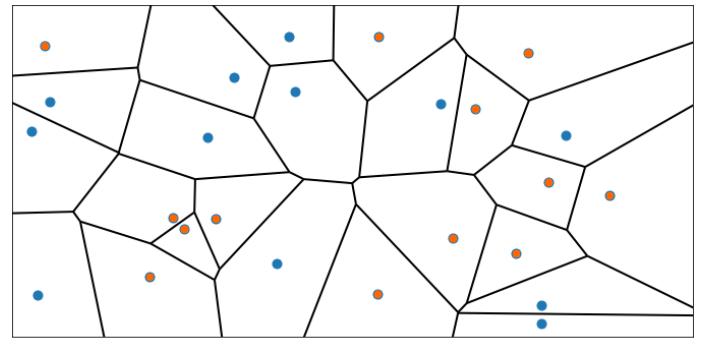
\includegraphics[width=0.75\textwidth]{Images/voronoiC.png}
%		
%		%\vspace*{0.3em}
%		\footnotesize{\textcolor{MPTgrey}{Diagramme de Voronoï\\ Tirée de l'ouvrage \textit{\href{http://cazencott.info/dotclear/public/lectures/IntroML_Azencott.pdf}{Introduction au Machine Learning}} de Chloé-Agathe Azencott} }
%	\end{center}
%}
%
%\only<2>{
%	\begin{center}
%		
%		
%		
%		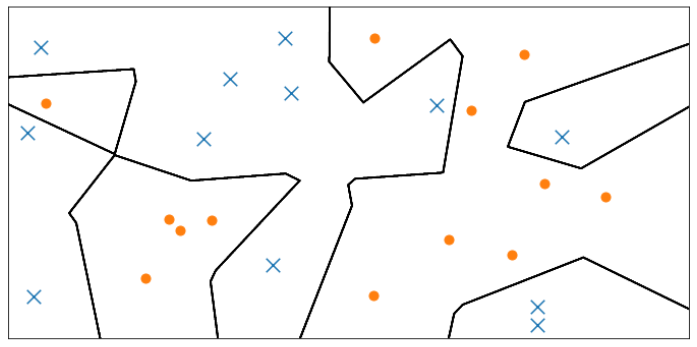
\includegraphics[width=0.75\textwidth]{Images/1NN.png}
%		
%		%\vspace*{0.3em}
%		\footnotesize{\textcolor{MPTgrey}{Frontière de décision du $\color{MPTgrey}1$NN\\ Tirée de l'ouvrage \textit{\href{http://cazencott.info/dotclear/public/lectures/IntroML_Azencott.pdf}{Introduction au Machine Learning}} de Chloé-Agathe Azencott} }
%	\end{center}
%}
%
%
%
%
%\end{frame}
%
%%------------------------------------------------------------------------------------------
%%------------------------------------------------------------------------------------------
%
%\begin{frame}{Exemples - $\color{MPTblue} \mathbf{1}$NN et $\color{MPTblue} \mathbf{15}$NN}
%
%\begin{itemize}
%	\item $\Y=\{0,1\}$\\[1.7em]
%\end{itemize}
%
%\begin{center}
%	
%	\begin{tikzpicture}
%		\node (ref) [base] {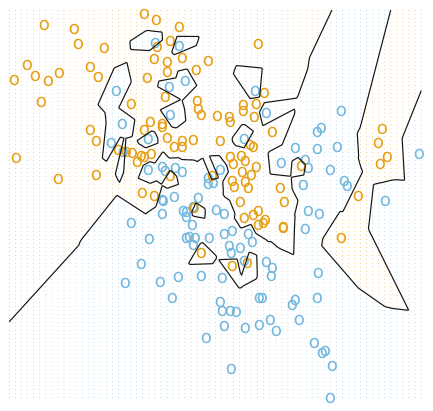
\includegraphics[width=0.4\textwidth,clip]{Images/1NN_1.png}};
%		\node (wiki)[]  at([yshift = 10]ref.north) {$K=1$};
%		\node (ref1) [base, right=of ref] {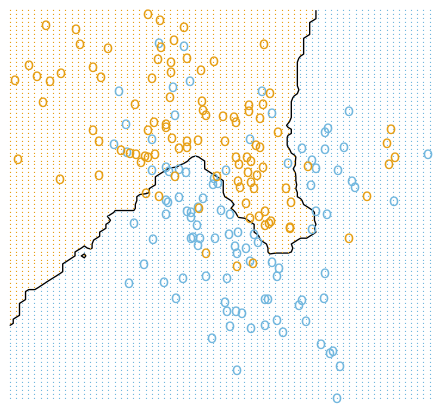
\includegraphics[width=0.4\textwidth,clip]{Images/15NN.png}};
%		\node (wiki)[]  at([yshift = 10]ref1.north) {$K=15$};
%	\end{tikzpicture}
%	
%	\vspace*{0.3em}
%	\footnotesize{\textcolor{MPTgrey}{Frontières de décision des $\color{MPTgrey}K$NN\\ Tirée de l'ouvrage \textit{\href{https://link.springer.com/book/10.1007/978-0-387-84858-7}{The Elements of Statistical Learning}}} }
%	
%\end{center}
%
%
%
%\end{frame}

%------------------------------------------------------------------------------------------
%------------------------------------------------------------------------------------------
%
%\begin{frame}{Qualités et défauts}
%
%L'algorithme des $K$ plus proches voisins : \\[2.3em]
%\begin{itemize}
%	\item[\smiley] simple à implémenter\\[1em]
%	\item[\smiley] méthode non-paramétrique : pas d'hypothèses particulières sur le modèle\\[1em]
%	\item[\smiley] s'adapte à tous types de données\\[2em]
%	\item[\frownie] intensif en temps de calcul : il faut calculer $n$ distances (compléxité de l’ordre de $O(nd)$ avec dim($\X)= d$) puis trouver les $K$ plus petites de ces distances (compléxité de l’ordre de $O(n \log K)$)\\[1em]
%	\item[\frownie] susceptible de ne pas marcher en grande dimension, \ie quand $d$ est grand (fléau de la dimension) \textcolor{MPTgrey}{--- \textit{Pourquoi ?}}\\[3em]
%\end{itemize}
%
%
%
%
%
%\end{frame}


%------------------------------------------------------------------------------------------
%------------------------------------------------------------------------------------------

\subsubsection{Minimisation empirique de l'erreur}

%------------------------------------------------------------------------------------------
%------------------------------------------------------------------------------------------

\begin{frame}{Risque empirique}
	\vspace*{-1.3em}
	\begin{minipt}[1]{0.15}

\bftitle{Contexte} \hsp On observe des {données} $x_1,\dots,x_n \in \X$ pour $n$ individus ainsi que des\\
\phantom{\bftitle{Contexte} \hsp} {étiquettes} $y_1,\dots,y_n \in \Y$ associées
\end{minipt}
\begin{minipt}[1]{0.84}
%	\vspace*{-.4em}
	\begin{minipc}[0.06]{0.11}
	\warning
\end{minipc}
%	\vspace*{-.4em}
\begin{minipt}[0.93]{0.11}
 $ {f^*= \text{{arg}}\,\min\limits_{f \in \F}\, R(f) = \text{{arg}}\,\min\limits_{f \in \F}\,\mathbb{E}_{\mathbb{P}_{X,Y}} \left[\ell\left(Y,f(X)\right)\right] }$ est \textbf{inconnue}
\end{minipt}
\pause
\begin{minipc}[0.06]{0.08}
		%\begin{center}
		\raisebox{1.5mm}{\bclampe \xspace} 
	\end{minipc}
	\begin{minipc}[0.93]{0.08}
		On va utiliser les données observées $(x_1,y_1), \dots, (x_n, y_n)$ pour approcher $R(f)$ par son estimation empirique donnée par		 
	\end{minipc}
%	\vspace*{-.3em}
$$ \dfrac{1}{n} \sum_{i=1}^n \ell\left(y_i, f(x_i)\right)$$
\vspace*{1em}

%	\vspace*{-.3em}
\pause
\bftitle{Objectif} \hsp Ainsi, on cherche $\hat{f}^*$ telle que $ \hat{f}^*= \text{{arg}}\,\min\limits_{f \in \F}\, \dfrac{1}{n} \displaystyle \sum_{i=1}^n \ell\left(y_i, f(x_i)\right)$\\[1.5em]
\pause

%	\vspace*{-.3em}
\bftitle{Remarque} \hsp Plus le nombre d'observation est grand, meilleure est l'estimation\\\phantom{\bftitle{Remarque} \hsp}empirique de $R(f)$

%\bftitle{Remarque} \hsp En pratique, on cherche $\hat{f}^*$ dans un sous ensemble $\H \subset \F$ car pour\\\phantom{\bftitle{Remarque} \hsp}certaines raisons (nature du problème, éviter le surapprentissage)\\\phantom{\bftitle{Remarque} \hsp} on pense qu'il est préférable de restreindre notre recherche à $\H$.\\\phantom{\bftitle{Remarque} \hsp}Le choix de $\H$ représente donc une information a priori ; on appelle\\\phantom{\bftitle{Remarque} \hsp}cela un \textbf{biais inductif } \\
%\phantom{\bftitle{Remarque} \hsp}\textcolor{MPTgrey}{ex : les prédicteurs linéaires ($\color{MPTgrey} \X = \bbR^d$)}\\
%\phantom{\bftitle{Remarque} \hsp}$\color{MPTgrey} \H = \left\{ f : x\in \bbR^d \mapsto \phi \left(\langle a,x \rangle + b\right), \, \, \phi : \bbR \to \Y,  a \in \bbR^d, b \in \bbR \right\}$
\end{minipt}	
\end{frame}
%----------------------------------------------------------------------------------------------------------------------------------------------------------

\begin{frame}{Risque empirique}
\vspace*{-1em}
		\bftitle{Objectif} \hsp On cherche $\hat{f}^*$ telle que $ \hat{f}^*= \text{{arg}}\,\min\limits_{f \in \F}\, \dfrac{1}{n}  \displaystyle \sum_{i=1}^n \ell\left(y_i, f(x_i)\right)$\\[1em]
		
	
		\pause
		En pratique, on cherche $\hat{f}^*$ dans un sous ensemble $\H \subset \F$ car pour certaines raisons (nature du problème, sur-apprentissage) on pense qu'il est préférable de restreindre notre recherche à $\H$. Le choix de $\H$ représente donc une information a priori ; on appelle cela un \textbf{biais inductif } \\[1.5em]
	%	\textcolor{MPTgrey}{ex :} $\color{MPTgrey} \H = \left\{ f : x\in %\bbR^d \mapsto \phi \left(\langle a,x \rangle + b\right), \, \, \phi : \bbR \to \Y,  a \in \bbR^d, b \in \bbR \right\}$ \, $(\color{MPTgrey}  \X \in \bbR^d)$\\
		
		
			\begin{minipage}[c][6cm][t]{0.17\textwidth}
			\bftitle{Exemple} 
		\end{minipage}
		\begin{minipage}[c][6cm][t]{0.81\textwidth}
		$ \H = \left\{ f : x\in \bbR^d \mapsto \phi \left(\langle a,x \rangle + b\right), \, \, \phi : \bbR \to \Y,  a \in \bbR^d, b \in \bbR \right\}$ \, $\color{MPTgrey}  (\X \in \bbR^d)$\\
		
		Si $\phi =$ fonction identité : \pause régression linéaire\\
		
		On cherche alors  $ \left(\widehat{a},\widehat{b}\right)= \text{{arg}}\,\min\limits_{a \in \bbR^d \, b \in \bbR}\, \dfrac{1}{n}  \displaystyle \sum_{i=1}^n \ell\left(y_i, \langle a,x_i \rangle + b\right)$\\[1em]
		
		Les solutions $\widehat{a}$ et $\widehat{b}$ s'expriment en fonction des données $(x_1,y_1), \dots, (x_n, y_n)$ : les données permettent donc \textit{d'apprendre}/ \textit{d'estimer} un modèle
		\end{minipage}
		
		
	
	
	\note{dire qu'on verra ça au second semestre pour le choix de H. Dire aussi AIC, BIC pourquoi ici on ne l'a pas ?
	
	préciser REG + remarque KNN + Pas que ERM : SRM et MDL (voir qui est quoi SVM : ERM, reg log : ERM, et arbre ?)}
\end{frame}

%--------------------------------------------------------------
\begin{frame}{Estimateur empirique du risque}
	\vspace*{-1em}
	$$\hat{f}^*= \text{{arg}}\,\min\limits_{f \in \H}\, \dfrac{1}{n} \sum_{i=1}^n \ell\left(y_i, f(x_i)\right)$$
	
	\vspace*{0.5em}
	\bftitle{Remarque} \hsp 	On utilise les données $(x_1,y_1), \dots, (x_n, y_n)$ car on fait l'hypothèse\\\phantom{\bftitle{Remarque} \hsp} qu'elle peuvent être modélisées par des vecteurs aléatoires\\\phantom{\bftitle{Remarque} \hsp} $(X_1,Y_1), \dots, (X_n, Y_n) \underset{\text{i.d.d.}}{\sim} \mathbb{P}_{X,Y}$\\[1.3em] 	
			
Modéliser $(x_1,y_1), \dots, (x_n, y_n)$ par des vecteurs aléatoires $(X_1,Y_1), \dots, (X_n, Y_n)$ nous permet de prendre en compte l'incertitude lié à l'échantillonnage (choix des $x_i$) et l'incertitude sur les étiquettes $y_i$ sachant les données $x_i$\\[1.7em] 

On introduit ainsi \textbf{l'estimateur empirique du risque} $\boldsymbol{ R_n(f)}$ défini par
$$ R_n(f) = \dfrac{1}{n} \sum_{i=1}^n \ell\left(Y_i, f(X_i)\right)$$

On peut alors s'intéresser aux propriétés des var. aléatoires $R_n(f)$ et 
$\text{{arg}}\,\min\limits_{f \in \H}\, R_n(f)$\\[2em]
		
		
\end{frame}

%------------------------------------------------------------------------------------------
%\begin{frame}
%
%\end{frame}
%------------------------------------------------------------------------------------------
%------------------------------------------------------------------------------------------
%------------------------------------------------------------------------------------------

%\subsection{Algorithme des plus proches voisins\\ \vspace{-0.5em} \normalsize une approche non-paramétrique}

%------------------------------------------------------------------------------------------
%------------------------------------------------------------------------------------------

%------------------------------------------------------------------------------------------
%------------------------------------------------------------------------------------------
%------------------------------------------------------------------------------------------
%------------------------------------------------------------------------------------------

\subsubsection{Évaluer un modèle}

%------------------------------------------------------------------------------------------
%------------------------------------------------------------------------------------------

\begin{frame}{Les métriques}
	\bftitle{Contexte} \hsp On observe des {données} $x_1,\dots,x_n \in \X$ pour $n$ individus ainsi que\\ \phantom{\bftitle{Contexte} \hsp}des {étiquettes} $y_1,\dots,y_n \in \Y$ associées\\[2em]
	
	\phantom{\bftitle{Contexte} \hsp} À l'aide des données, on a appris un modèle $f$\\[1em]
	\phantom{\bftitle{Contexte} \hsp}\textcolor{MPTgrey}{\ex} $\color{MPTgrey} \hsp f(x) = \text{\textcolor{MPTgrey}{arg}}\, \displaystyle \max\limits_{k \in \Y}\, \sum_{i  : x_i \in \N_K(x) } \mathbb{1}\left\{y_i = k\right\} \hsp x \in \X$\\[1em]
		\phantom{\bftitle{Contexte} \hsp}\textcolor{MPTgrey}{\ex} $\color{MPTgrey} \hsp f(x) = \langle \hat{a},x \rangle + \hat{b}\hsp x \in \X$\\[1.5em]
	
	\bftitle{Question} \hsp Quelles sont les performances de $f$ ?\\[2em]
	
	\bftitle{Définition}
	\begin{vblock}{}
		Une \textbf{métrique} est un score qui permettra d’évaluer les performances d'un modèle	
	\end{vblock}
	\, \ex \, Les métriques choisies vont dépendre des données, du modèle et de la
	\phantom{\, \ex \,}problématique
	
\end{frame}

%------------------------------------------------------------------------------------------
%------------------------------------------------------------------------------------------


%------------------------------------------------------------------------------------------


%------------------------------------------------------------------------------------------

\begin{frame}{Les métriques - classification binaire}
	\vspace*{-1.8em}
	\begin{itemize}
		\item $\Y = \{0,1\}$\\[1em]
	\end{itemize}
	
	
	\begin{center}
		\bftitle{Matrice de confusion} \\[1em]
		\begin{table}[h!]
			\centering
			\begin{tabular}{|c|c|c|c|}
				\hline
				\multicolumn{2}{|c|}{} & \multicolumn{2}{c|}{Classe réelle} \\ \hline
				\multicolumn{2}{|c|}{} & 0 & 1 \\ \hline
				\multirow{2}{*}{Classe prédite} & 0 & vrais négatifs (TN) & faux négatifs (FN) \\ \cline{2-4} 
				& 1 & faux positifs (FP) & vrais positifs (TP) \\ \hline
			\end{tabular}
		\end{table}
		%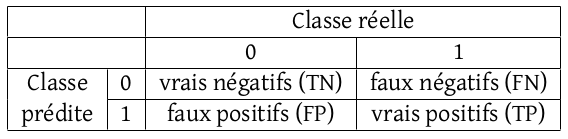
\includegraphics[width=0.8\textwidth]{Images/confusion2.png}
	\end{center}
	\vspace{0.5em}
	\begin{itemize}
		\item \textbf{Vrais positifs (TP)} : exemples positifs correctement classifiés par le modèle\\[0.3em]
		\item \textbf{Vrais négatifs (TN)} : exemples négatifs correctement classifiés par le modèle\\[0.3em]
		\item \textbf{Faux positifs (FP)} : exemples négatifs étiquetés positifs par le modèle\\[0.3em]
		\item \textbf{Faux négatifs (FN)} : exemples positifs étiquetés négatifs par le modèle\\[0.3em]
	\end{itemize}
	\vspace*{2em}
	\clrcite{TP : True Positives \hfill TN : True Negatives \hfill FP : False Positives \hfill FN : False Negatives}
	
	\note{Faire TP mais avant + dire autre métrique quand ne renvoie pas une étiquette : voir courbe ROC régression logistique + dans TP IRIS, ça serait cool de faire macro-average}
\end{frame}

%------------------------------------------------------------------------------------------

%------------------------------------------------------------------------------------------

%------------------------------------------------------------------------------------------

\begin{frame}{Les métriques - classification binaire}
	\vspace*{-.8em}
	\begin{itemize}
		\item $\Y = \{0,1\}$\\[2em]
	\end{itemize}
	
	\bftitle{Accuracy} \hsp Proportion d’exemples bien classés\\
	\pause
	$$ \text{Accuracy } = \dfrac{\text{TP} + \text{TF}}{\text{TP}+\text{TF}+\text{FP}+\text{FN}}$$
	
	\pause
	\begin{minipc}[0.06]{0.18}
		\warning
	\end{minipc}
	\begin{minipc}[0.93]{0.18}
		 
	\end{minipc}
	
Utiliser l'accuracy comme métrique principale pour évaluer un modèle de classification peut poser problème lorsqu'on a des données déséquilibrées car elle ne reflète pas la capacité du modèle à bien classer la classe minoritaire, qui peut-être la classe "de plus grande importance".
\end{frame}
%------------------------------------------------------------------------------------------


%\begin{frame}{Les métriques - classification binaire}
%	\vspace*{-.8em}
%	\begin{itemize}
%		\item $\Y = \{0,1\}$\\[2em]
%	\end{itemize}
%	
%	\bftitle{Rappel ou Sensibilité} \hsp Proportion d’exemples positifs correctement\\\phantom{\bftitle{Rappel ou Sensibilité} \hsp }classifiés, \ie taux de vrais positifs\\
%	$$ \text{Sensibilité } = \dfrac{\text{TP}}{\text{TP}+\text{FN}}$$
%	
%	
%	\begin{minipc}[0.06]{0.18}
%		\warning
%	\end{minipc}
%	\begin{minipc}[0.93]{0.18}
%		Il est facile d’avoir une bonne sensibilité en prédisant que tous les exemples sont positifs. On regarde donc aussi la précision	 
%	\end{minipc}
%	
%	\vspace{1em}
%	\bftitle{Précision} \hsp Proportion de prédictions correctes parmi les prédictions positives\\
%	$$ \text{Précision } = \dfrac{\text{TP}}{\text{TP}+\text{FP}}$$
%	
%	%	\phantom{\bftitle{Précision} \hsp} \textbf{La précision peut aussi se calculer pour une classification\\\phantom{\bftitle{Précision} \hsp} multi-classe}
%	\vspace{0.5em}
%		\begin{minipc}[0.06]{0.18}
%		\warning
%	\end{minipc}
%	\begin{minipc}[0.93]{0.18}
%	On peut avoir une bonne précision (au détriment du rappel) en faisant très peu de prédictions positives car cela réduit le risque qu’elles soient erronées		 
%	\end{minipc}
%%	\textbf{Remarque} : On peut avoir une bonne précision (au détriment du rappel) en faisant très peu de prédictions positives car cela réduit le risque qu’elles soient erronées	
%\end{frame}

%------------------------------------------------------------------------------------------

\begin{frame}{Les métriques - classification binaire}
	\vspace*{-.8em}
	\begin{itemize}
		\item $\Y = \{0,1\}$\\[2em]
	\end{itemize}
	
	\bftitle{Rappel ou Sensibilité} \hsp Proportion d’exemples positifs correctement\\\phantom{\bftitle{Rappel ou Sensibilité} \hsp }classifiés, \ie taux de vrais positifs\\
	$$ \text{Sensibilité } = \dfrac{\text{TP}}{\text{TP}+\text{FN}}$$
	
	
	\begin{minipc}[0.06]{0.18}
		\warning
	\end{minipc}
	\begin{minipc}[0.93]{0.18}
		Il est facile d’avoir une bonne sensibilité en prédisant que tous les exemples sont positifs. On regarde donc aussi la précision	 
	\end{minipc}
	
	\vspace{1em}
	\bftitle{Précision} \hsp Proportion de prédictions correctes parmi les prédictions positives\\
	$$ \text{Précision } = \dfrac{\text{TP}}{\text{TP}+\text{FP}}$$
	
	%	\phantom{\bftitle{Précision} \hsp} \textbf{La précision peut aussi se calculer pour une classification\\\phantom{\bftitle{Précision} \hsp} multi-classe}
	\vspace{0.5em}
	\begin{minipc}[0.06]{0.18}
		\warning
	\end{minipc}
	\begin{minipc}[0.93]{0.18}
		On peut avoir une bonne précision (au détriment du rappel) en faisant très peu de prédictions positives car cela réduit le risque qu’elles soient erronées		 
	\end{minipc}
	%	\textbf{Remarque} : On peut avoir une bonne précision (au détriment du rappel) en faisant très peu de prédictions positives car cela réduit le risque qu’elles soient erronées	
\end{frame}
%------------------------------------------------------------------------------------------



\begin{frame}{Les métriques - classification binaire}
	\vspace*{-1em}
	\begin{itemize}
		\item $\Y = \{0,1\}$\\[2em]
	\end{itemize}
	
	\bftitle{F-mesure ou F1-score} \hsp Moyenne harmonique
	de la précision et du rappel\\
	$$ \text{F1-score } = 2 \dfrac{\text{Précision} \cdot \text{Rappel} }{\text{Précision} +\text{Rappel} } = \dfrac{2\text{TP}}{2\text{TP}+\text{FP}+\text{FN}}$$
	\vspace{4em}
	
	\bftitle{Spécificité} \hsp Proportion d’exemples négatifs correctement classifiés, \ie le taux  de vrais négatifs\\
	$$ \text{Spécificité } = \dfrac{\text{TN}}{\text{FP}+\text{TN}}$$
	
	%	\phantom{\bftitle{Spécificité} \hsp} \textbf{La spécificité peut aussi se calculer pour une classification\\\phantom{\bftitle{Précision} \hsp} multi-classe}
	\begin{minipc}[0.06]{0.18}
	\warning
\end{minipc}
\begin{minipc}[0.93]{0.18}
	Il est facile d’avoir une bonne spécificité en prédisant que tous les exemples sont négatifs. Il est donc également intéressant de regarder la spécificité et la sensibilité en même temps.	 
\end{minipc}
	\note{parler courbe ROC
	pour moyenne harmonique : C'est l'inverse de la moyenne arithmétique des inverses des termes. La moyenne harmonique est donc utilisée lorsqu'on veut déterminer un rapport moyen, dans un domaine où il existe des liens de proportionnalité inverses.  Le F1-score étant une moyenne harmonique de la précision et du recall, il n'est élevé qu'à condition que ces deux indicateurs soient élevés. Il traduit donc bien un compromis entre precision et recall.
	
	Par exemple, les scores F1 utilisent une moyenne harmonique pour favoriser des valeurs de précision et de rappel similaires : si l’une est bien inférieure à l’autre, le score F1 sera inférieur à ce qu’il serait s’il s’agissait simplement de la moyenne arithmétique de précision et de rappel}
\end{frame}

%------------------------------------------------------------------------------------------
%------------------------------------------------------------------------------------------

%------------------------------------------------------------------------------------------



\begin{frame}{Les métriques - classification binaire}
	\vspace*{-1em}
	\begin{itemize}
		\item $\Y = \{0,1\}$\\[3em]
	\end{itemize}
	
	\bftitle{AUC} \hsp L'aire sous la courbe ROC\\[1em]

	Elle mesure la capacité du modèle à séparer correctement les classes. \\[1em]
	
	La courbe ROC et l'AUC seront présentés dans la partie sur la régression logistique (partie suivante)\\[10em]
\end{frame}

%------------------------------------------------------------------------------------------
%------------------------------------------------------------------------------------------
\begin{frame}{Les métriques - classification multiclasse}
	\vspace*{-1.2em}
	\begin{itemize}
		\item $\Y = \{1, \dots, C\}$\\[1.5em]
	\end{itemize}
	
	\bftitle{Matrice de confusion} \hsp Matrice $M$ avec $C$ lignes et $C$ colonnes et où $M_{i,j}$\\\phantom{\bftitle{Matrice de confusion} \hsp}représente le nombre d’exemples de la classe $i$ pour\\\phantom{\bftitle{Matrice de confusion} \hsp} laquelle l’étiquette $j$ a été prédite\\[1em]
	
	\begin{center}
		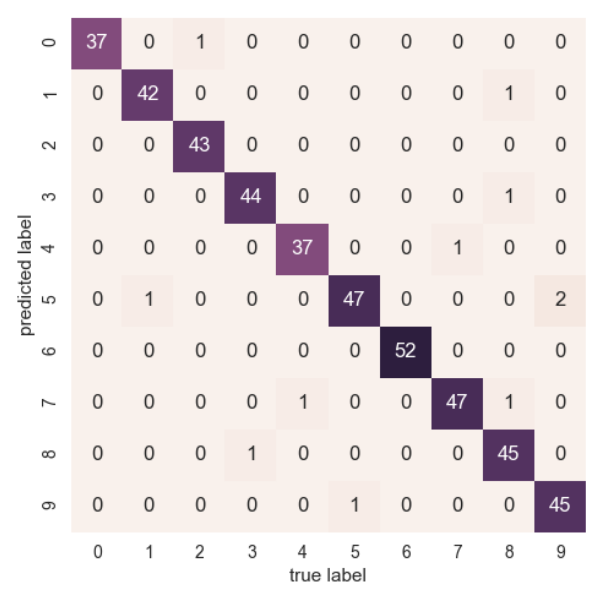
\includegraphics[width=0.47\textwidth]{Images/confusionC.png}
	\end{center}
	
	
\end{frame}
%------------------------------------------------------------------------------------------
%------------------------------------------------------------------------------------------

\begin{frame}{Les métriques - classification multiclasse}
	\only<1>{	\vspace*{-1.3em}
		\begin{itemize}
			\item $\Y = \{1,\dots, C\}$\\[1em]
		\end{itemize}
		
		On peut calculer les métriques précédentes pour chaque classe $i \in \{1,\dots, C\}$ en considérant que les autres classes forment une seule et même classe (stratégie One Versus All). On combine ensuite les métriques $m_i$ de chaque classe pour obtenir un score global\\[1em]
		
		\bftitle{Macro-average} \hsp  $\texttt{macro\_average\_}\textit{score}=\frac{1}{C}\sum_{i=1}^C m_i$\\[0.2em]
		\phantom{\bftitle{Macro-average} \hsp }Permet de ne pas négliger les classes rares\\[1em]
		
		\bftitle{Weight-average} \hsp  $\texttt{weight\_average\_}\textit{score}=\sum_{i=1}^C \frac{m_i \ \times \text{ support}_i}{\text{nb. données total}}$\\[0.2em]
		\phantom{\bftitle{Weight-average} \hsp }Chaque classe est pondérée par son support, \ie le\\\phantom{\bftitle{Weight-average} \hsp}nombre d'observations dans cette classe. Les classes\\\phantom{\bftitle{Weight-average} \hsp} très représentées ont beaucoup de poids    \\[1em]
		
		\bftitle{Micro-average} \hsp Correspond à l'accuracy, i.e. la proportion d'exemple bien\\\phantom{\bftitle{Micro-average} \hsp}classés.
		
%		On calcule le nombre de TP, FN et FP au global. Cela revient à\\\phantom{\bftitle{Micro-average} \hsp}regarder l'\textit{accuracy} qui est la proportion d’exemples\\\phantom{\bftitle{Micro-average} \hsp}correctement étiquetés. Chaque élément du jeu de données\\\phantom{\bftitle{Micro-average} \hsp}ayant la même importance, les classes très représentées ont\\\phantom{\bftitle{Micro-average} \hsp}beaucoup de poids. Voir \eg \href{https://simonhessner.de/why-are-precision-recall-and-f1-score-equal-when-using-micro-averaging-in-a-multi-class-problem/}{ce site}   
	}
	\only<2>{\begin{center}
			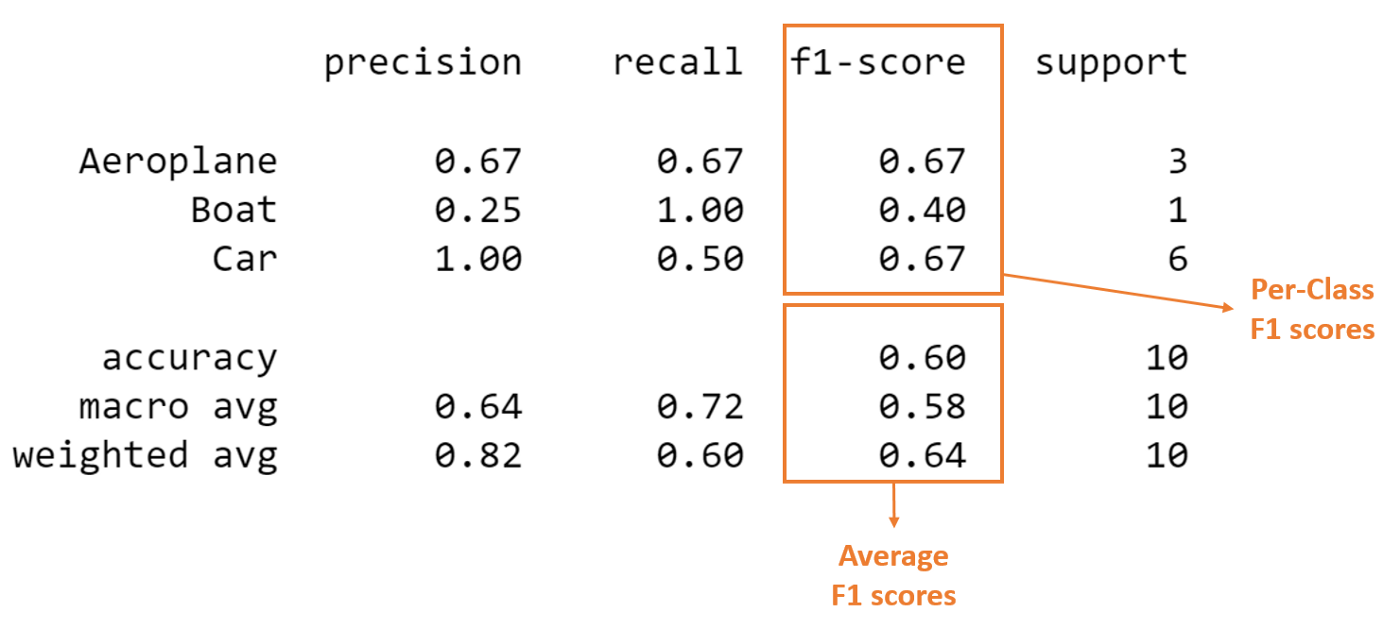
\includegraphics[width=0.9\textwidth]{Images/average.png}
		\end{center}
	}
	\note{faire exercice https://datascience.stackexchange.com/questions/15989/micro-average-vs-macro-average-performance-in-a-multiclass-classification-settin et inverse exemple ensuite : classes A, C, D : 0 TP et 2 FP et classe B : 90 TP et 10 FP}
\end{frame}

%------------------------------------------------------------------------------------------
\begin{frame}{Les métriques - Classification multiclasse}

	
	\begin{center}
	\bftitle{Exercice} \\[1em]
	\begin{table}[h!]
		\centering
		\begin{tabular}{|c|c|c|c|c|}
			\hline
		%	\multicolumn{2}{|c|}{} & \multicolumn{2}{c|}{Classe réelle} \\ \hline
			& \multicolumn{2}{c|}{Situation 1} & \multicolumn{2}{c|}{Situation 2} \\ \hline
			& TP&FP&TP&FP\\\hline
			 Classe A & 1 & 1  & 0 &2  \\
			 Classe B & 10 &90  & 90 & 10  \\
			  Classe C& 1 & 1  & 0 &2  \\
			   Classe D & 1 & 1  & 0 &2  \\
			 \hline
		\end{tabular}
	\end{table}
	%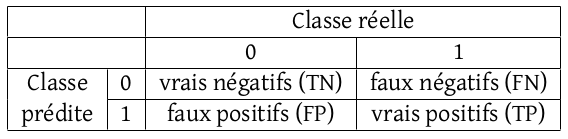
\includegraphics[width=0.8\textwidth]{Images/confusion2.png}
\end{center}

\vspace*{1em}
Pour chacune des situation : \\[0.5em]
\begin{enumerate}
	\item Calculer la précision de cette classification multiclasse via la méthode du macro-average puis celle du micro-average\\[0.3em]
	\item Commenter les résultats : quelle différence observe-t-on entre la méthode macro-average et  micro-average ?
\end{enumerate}

\vspace{2em}

\end{frame}
%------------------------------------------------------------------------------------------
%------------------------------------------------------------------------------------------

\


%------------------------------------------------------------------------------------------
\begin{frame}{Les métriques - régression}
	\bftitle{MSE (Mean Square Error) : la moyenne des erreurs }
	
	$$ \text{MSE} = \dfrac{1}{n} \sum_{i=1}^n \left(y_i - \widehat{f}(x_i)\right)^2$$
	
	\vspace*{3em}
	\bftitle{RMSE (Root Mean Square Error)  }
	
	$$ \text{RMSE } = \sqrt{\dfrac{1}{n} \sum_{i=1}^n \left(y_i - \widehat{f}(x_i)\right)^2}$$
	\note{parler de AIC mais ils n'ont pas encore fait le cours. DIRE AUSSI COMPARER A MODELE NAIF}
\end{frame}
%------------------------------------------------------------------------------------------
%------------------------------------------------------------------------------------------

\subsubsection{Sur-apprentissage et dilemme biais-variance}

\begin{frame}{Capacité de généralisation}
	
		\bftitle{Contexte} \hsp On observe des {données} $x_1,\dots,x_n \in \X$ ainsi que des {étiquettes}\\
	\phantom{\bftitle{Objectif} \hsp}$y_1,\dots,y_n \in \Y $ et l'on souhaite estimer l'étiquette d'une nouvelle\\\phantom{\bftitle{Objectif} \hsp} observation $x \in \X$\\[1em]
	
	\bftitle{Exemple}\\
	\vspace*{-0.2em}
	\begin{vexblock}{}
	On considère l'algorithme dont la règle de décision est donnée par 
	$$ f(x) = \left\{\begin{array}{l}
		y_i \hsp \hsp  \text{ si } x=x_i  \text{ pour }   i \in \llbracket1,n \rrbracket\\
		y \in \Y \text{ choisi aléatoirement} \hsp \hsp  \text{sinon}		
	\end{array} \right.$$ 
Cet algorithme aura
	une erreur empirique nulle quelle que soit la fonction de coût $\ell$ choisie.
	$$\dfrac{1}{n} \sum_{i=1}^n \ell\left(y_i, f(x_i)\right) = 0,$$ 
	Il fait donc de bonnes prédictions sur les données utilisées pour le construire (il aura de très bonnes performances sur ces données) mais fera de très mauvaises prédictions pour toute nouvelle observation.
	\end{vexblock}
	
\end{frame}

%------------------------------------------------------------------------------------------
%------------------------------------------------------------------------------------------

\begin{frame}{Capacité de généralisation}
	
	\vspace*{-0.5em}
	\bftitle{Définition}\\
	\vspace*{-0.1em}
	\begin{vblock}{}\itshape
On appelle \textbf{capacité de généralisation} la capacité d’un modèle à faire des prédictions correctes sur de nouvelles données, qui n’ont pas été utilisées pour le construire
	\end{vblock}
	\vspace*{-0.1em}
Deux cas où les modèles généralisent mal :\\[0.8em]
\begin{itemize}
	\item \bftitle{Sur-apprentissage} : le modèle, plutôt que de capturer la nature des objets à étiqueter, modélise aussi le bruit et ne sera pas en mesure de généraliser\\ \textbf{On dit que le modèle sur-apprend} \\[0.5em]
	
	Un modèle qui sur-apprend est généralement un modèle trop complexe, qui \textit{colle} trop aux données car il a aussi capturé leur bruit\\[1em]
	\item \bftitle{Sous-apprentissage} : le modèle est trop simple pour avoir de bonnes performances même sur les données utilisées pour le construire\\ \textbf{On dit que le modèle sous-apprend}.
\end{itemize}

\vspace*{0.8em}
\bftitle{Remarque} \hsp Les données peuvent être bruitées par des erreurs de mesure,\\
\phantom{\bftitle{Remarque} \hsp}des erreurs d'étiquetage ou parce que les variables mesurées ne\\
\phantom{\bftitle{Remarque} \hsp}suffisent pas à modéliser le phénomène qui nous intéresse
\end{frame}

%------------------------------------------------------------------------------------------
%------------------------------------------------------------------------------------------

%pour définir des couleurs utilisées dans le tikz
\definecolor{amethyst}{rgb}{0.6, 0.4, 0.8}
\definecolor{alizarin}{rgb}{0.82, 0.1, 0.26}
\definecolor{amber}{rgb}{1.0, 0.49, 0.0}
\definecolor{ao}{rgb}{0.0, 0.5, 0.0}
\begin{frame}{Capacité de généralisation - Exemples}
	
	\begin{center}
		\begin{tikzpicture}
		\node(ref){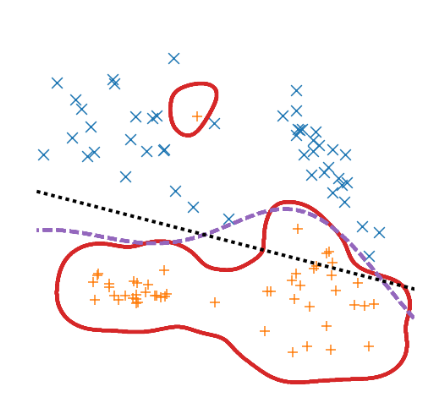
\includegraphics[width=0.49\textwidth]{Images/generalisation1.png}};		
		\node (text) [draw=alizarin,fill=white, thick,minimum width=1.5cm,minimum height=0.5cm,visible on=<2->] at(0.5,2) {\scshape \footnotesize \textcolor{alizarin}{sur-apprentissage}};
		\node (text) [draw=black,fill=white, thick,minimum width=1.5cm,minimum height=0.5cm,visible on=<3->] at(-1,0.4) {\scshape \footnotesize \textcolor{black}{sous-apprentissage}};
		\node (text) [draw=amethyst,fill=white, thick,minimum width=1.5cm,minimum height=0.5cm,visible on=<4->] at(1.5,0) {\scshape \footnotesize \textcolor{amethyst}{bon compromis}};
%
%
		\node (ref1) at([xshift =90]ref.east)
 {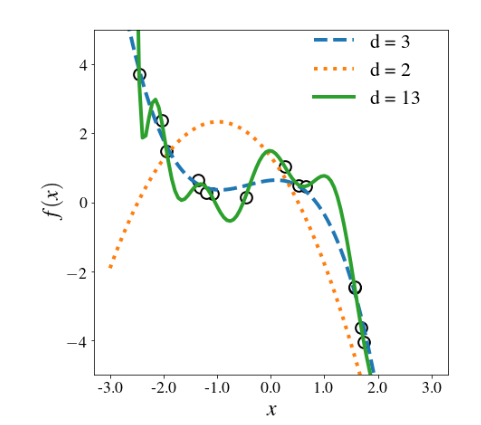
\includegraphics[width=0.49\textwidth]{Images/generalisation2.png}};
 		\node (text) [draw=amber,fill=white, thick,minimum width=1.5cm,minimum height=0.5cm,visible on=<5->] at(6.5,-1.5) {\scshape \footnotesize \textcolor{amber}{sous-apprentissage}};
 \node (text) [draw=ao,fill=white, thick,minimum width=1.5cm,minimum height=0.5cm,visible on=<6->] at(6,1.9) {\scshape \footnotesize \textcolor{ao}{sur-apprentissage}};
 \node (text) [draw=MPTblue,fill=white, thick,minimum width=1.5cm,minimum height=0.5cm,visible on=<7->] at(6.3,-0.5) {\scshape \footnotesize \textcolor{MPTblue}{bon compromis}};

	\end{tikzpicture}

\vspace*{1em}
		\footnotesize{\textcolor{MPTgrey}{Images tirées de l'ouvrage \textit{\href{http://cazencott.info/dotclear/public/lectures/IntroML_Azencott.pdf}{Introduction au Machine Learning}} de Chloé-Agathe Azencott} }
\end{center}


		
\vspace*{2em}
\end{frame}

%------------------------------------------------------------------------------------------
%------------------------------------------------------------------------------------------

\begin{frame}{Capacité de généralisation - Exemples}
	

	\begin{center}
		
		\begin{tikzpicture}
			\node (ref) [base] {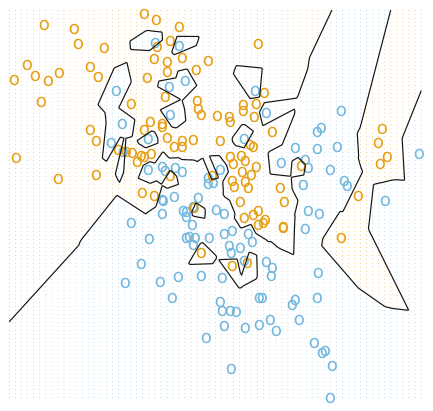
\includegraphics[width=0.4\textwidth,clip]{Images/1NN_1.png}};
			\node (wiki)[]  at([yshift = 10]ref.north) {$K=1$};
			\node (wiki)[draw=MPTgrey,fill=white, very thick,visible on=<2->]  at([yshift = 15]ref.south) {\textcolor{MPTgrey}{Sur-apprentissage}};
			
					\node (ref1) [base, right=of ref] {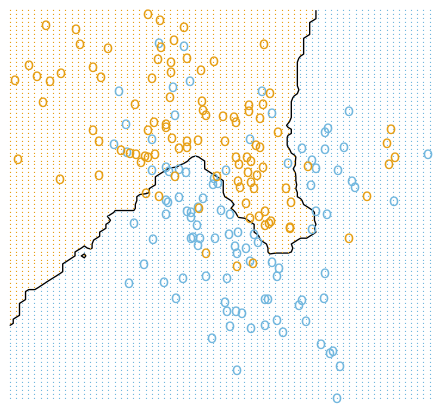
\includegraphics[width=0.4\textwidth,clip]{Images/15NN.png}};
			\node (wiki)[]  at([yshift = 10]ref1.north) {$K=15$};
			\node (wiki)[draw=MPTgrey,fill=white, very thick,visible on=<3->]  at([yshift = 15]ref1.south) {\textcolor{MPTgrey}{Bon compromis}};
		\end{tikzpicture}	
		
		\vspace*{0.3em}
		\footnotesize{\textcolor{MPTgrey}{Algorithme des $\color{MPTgrey}K$ plus proches voisins pour de la classification binaire\\
				Tirée de l'ouvrage \textit{\href{https://link.springer.com/book/10.1007/978-0-387-84858-7}{The Elements of Statistical Learning}}} }\\[1.5em]
		
	\end{center}


\begin{itemize}
	\item Et quand $K = n$ où  $n$ est le nombre de données observées ? \uncover<3->{\textcolor{MPTgrey}{Sous-apprentissage}}
\end{itemize}
	
	
	
\end{frame}

%------------------------------------------------------------------------------------------
%------------------------------------------------------------------------------------------

\begin{frame}{Compromis biais-variance avec les KNN}
	\vspace*{-0.5em}
	%\bftitle{Contexte} \hsp On observe $(x_1,y_1),\dots,(x_n,y_n) \in \bbR^d \times \{1,\dots,C\}$ modélisées par les\\\phantom{\bftitle{Contexte} \hsp}vecteurs aléatoires $(X_1,Y_1),\dots,(X_n,Y_n)$ à partir desquelles on\\\phantom{\bftitle{Contexte} \hsp} entraîne un modèle $\hat{f}$\\[1em]
	\bftitle{Contexte} \hsp On entraîne un algorithme des $K$ plus proches voisins à partir de\\\phantom{\bftitle{Contexte} \hsp}données observées $(x_1,y_1),\dots,(x_n,y_n) \in \bbR^d \times \{1,\dots,C\}$ et on\\\phantom{\bftitle{Contexte} \hsp}note $f$ le modèle résultant.\\[0.8em]


%	Soit $x \in \X$ une nouvelle donnée dont l'étiquette inconnue est $y \in \Y$. 
	La qualité du modèle $f$ va dépendre du \textit{\textbf{biais}} et de la \textit{\textbf{variance}} qui lui sont associés. On souhaiterait qu'ils soient les plus petits possible.  \\[1em]
	
	\bfblue{Le biais} de $f$ correspond en quelque sorte à la capacité de $f$ à bien prédire l'étiquette d'une nouvelle donnée $x$ : est-ce que $f(x)$ est loin ou non de sa vraie étiquette $y$ (inconnue) ? Plus $f(x)$ vise à côté de $y$, plus le biais est élevé\\[1em]
	
	\bfblue{La variance } de $f$ reflète la capacité du modèle à capturer le bruit dans les données et donc à sur-apprendre. Dans ce cas, on observe une forte variation de $f(x)$ en fonction des données d'entraînement $(x_1,y_1),\dots,(x_n,y_n)$\\[1em]

	
		\begin{minipc}[0.78]{0.15}
	\begin{itemize}
	\item $K$ diminue : \uncover<2->{la variance augmente, le biais diminue} \\[0.5em]
	\item $K$ augmente :  \uncover<3->{le biais augmente, la variance diminue}\\[0.8em]
\end{itemize}
	\end{minipc}
	\begin{minipc}[0.2]{0.15}
voir \href{https://mlu-explain.github.io/bias-variance/}{\textcolor{cyan}{ce site} (partie KNN en bas de page)}
	\end{minipc}
	
	
	\begin{valblock}{}
Lorsqu'on choisit $K$, il y a un \textbf{compromis} à faire entre le biais et la variance
	\end{valblock}
\note{montrer que erreur s'écrit en fonction du biais et de la variance ?
Site sympa pour biais variance trade off : https://mlu-explain.github.io/bias-variance/}
\end{frame}

%------------------------------------------------------------------------------------------
%------------------------------------------------------------------------------------------


%
%\begin{frame}{Compromis biais-variance}
%\bftitle{Rappel} \hsp $\F = \left\{ f : \X \to \Y  \, \text{ mesurable}\right\}$ et $\H$ : espace des hypothèses\\[0.8em]	
%\bftitle{Contexte} \hsp Soit un modèle $f \in \H \subset \F $ et le risque associé $R(f)$\\[0.5em]
%\phantom{\bftitle{Contexte} \hsp} On s'intéresse à \textbf{l'excès de risque} $\mathbf{R(f) - \displaystyle \inf_{h\in\mathcal{F}}R(h)}$ : \\[1em]
%
%	\vspace*{-0.5em}
%	
%%	\textbf{Décomposition de l'erreur de risque} $\mathbf{R(f) - \displaystyle \inf_{h\in\mathcal{F}}R(h)}$ :
%	$$R(f) \, \,  - \underbrace{\inf_{h\in\mathcal{F}}R(h)}_{\text{Erreur de Bayes}} = \underbrace{\left(\inf_{h\in\mathcal{H}}R(h)-\inf_{h\in\mathcal{F}}R(h)\right)}_{\text{Erreur d'approximation}}+\underbrace{\left(R(f)-\inf_{h\in\mathcal{H}}R(h)\right)}_{\text{Erreur d'estimation}}$$
%%	\vspace*{-0.3em}
%	\begin{itemize}
%		\item  \hsp \textbf{Erreur d'approximation} : quantifie la distance entre le modèle optimal sur \hsp $\H$ et celui sur $\F$ et donc la qualité du choix de $\H$ \hsp $ \color{MPTblue}\approx$ \bfblue{biais}
%		\item  \hsp \textbf{Erreur d'estimation} : quantifie la distance entre le modèle $f$ et le modèle \hsp optimal sur $\H$  \hsp $ \color{MPTblue}\approx$ \bfblue{variance}
%		\item \hsp  \textbf{Erreur de Bayes} : erreur irréductible\\[1.5em]
%	\end{itemize}
%
%\bftitle{Remarque} \hsp L'erreur d'estimation et d'approximation dépendent de la\\\phantom{\bftitle{Remarque} \hsp}complexité du modèle \textcolor{MPTgrey}{(\eg nombre de paramètres)}\\[1em]
%\end{frame}

%------------------------------------------------------------------------------------------
%------------------------------------------------------------------------------------------

\begin{frame}{Compromis biais-variance et compléxité}
	
		\begin{center}
		
		
		
		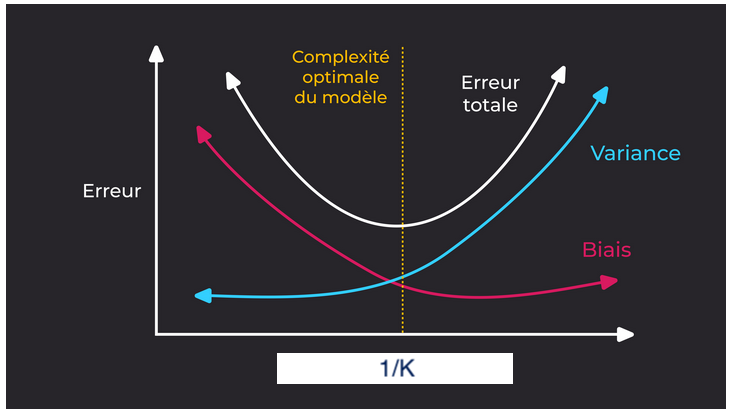
\includegraphics[width=0.9\textwidth]{Images/complexite1.png}
		
		\vspace*{0.3em}
		\footnotesize{\textcolor{MPTgrey}{Image trouvée sur \href{https://openclassrooms.com/fr/courses/4011851-initiez-vous-au-machine-learning/4092326-trouvez-le-bon-compromis-entre-biais-et-variance}{Open Classroom}}}
	\end{center}
%Complexité du modèle = \pause 
\end{frame}



\subsubsection{Sélectionner un modèle}

%------------------------------------------------------------------------------------------
%------------------------------------------------------------------------------------------

\begin{frame}{Jeu d'apprentissage et de test}
	\vspace*{-1em}
		\begin{minipc}[0.06]{0.18}
		\warning
	\end{minipc}
	\begin{minipc}[0.93]{0.18}
	\textbf{Sur-apprentissage} : un modèle peut faire de très bonnes prédictions sur les données utilisées pour le construire mais de très mauvaises prédictions pour des nouvelles observations		 
	\end{minipc}
	\begin{minipc}[0.06]{0.2}
		%\begin{center}
		\raisebox{1.5mm}{\bclampe \xspace} 
	\end{minipc}
	\begin{minipc}[0.93]{0.2}
	Évaluer un modèle avec des données étiquetées qui n’ont pas servi
	à le construire. Pour cela on divise le jeu de données en un \textbf{jeu d'apprentissage} et un \textbf{jeu test} 
	\end{minipc}

\begin{itemize}
	\item \bfblue{Le jeu d'apprentissage} : Sous-ensemble des données sur lequel on va apprendre un modèle\\[0.5em] 
	\item \bfblue{Le jeu de test} : \textbf{Sous-ensemble des données sur lequel on va évaluer le modèle}. Il permettra de \textbf{sélectionner} un modèle parmi plusieurs modèles différents appris sur le jeu d'apprentissage. (Permet d'ajuster les hyperparamètres)
\end{itemize}

\begin{center}
	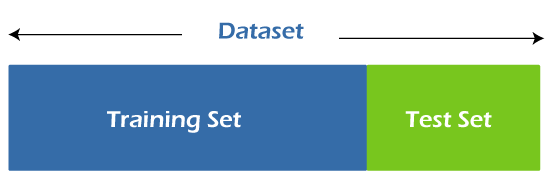
\includegraphics[width=0.55\textwidth]{Images/trainingset.png}
\end{center}
\end{frame}

%------------------------------------------------------------------------------------------
%------------------------------------------------------------------------------------------

\begin{frame}{Validation croisée}
	\vspace*{-1em}
	\begin{minipc}[0.06]{0.17}
		\warning
	\end{minipc}
	\begin{minipc}[0.93]{0.17}
		La séparation d’un jeu de données en un jeu d’entraînement et un jeu de test est arbitraire. Le risque est de créer, par hasard, des jeux de données qui ne sont pas représentatifs.	 
	\end{minipc}

\vspace*{-1em}
	\begin{minipc}[0.06]{0.18}
		%\begin{center}
		\raisebox{1.5mm}{\bclampe \xspace} 
	\end{minipc}
	\begin{minipc}[0.93]{0.18}
On pourrait reproduire plusieurs fois la procédure apprentissage/test puis moyenner les résultats obtenus
	\end{minipc}
	
\bftitle{Validation croisée}
\begin{enumerate}
	\item On divise le jeu de données en $M$ parties de tailles sensiblement similaires\\[0.1em]
	\item Pour chaque partie $i \in \llbracket 1,M\rrbracket$, on entraîne un même modèle sur l'ensemble des autres $M-1$ parties puis on évalue le modèle appris sur la partie $i$
	\item On moyenne les performances des $M$ modèles/prédicteurs appris
\end{enumerate}
	
	\begin{center}
		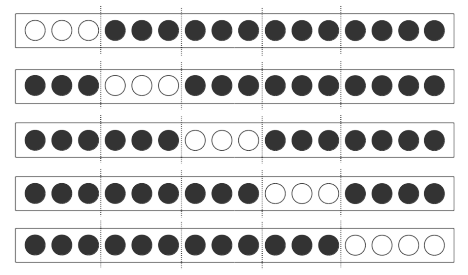
\includegraphics[width=0.35\textwidth]{Images/crossvalidation.png}
	\end{center}
\end{frame}

\begin{frame}
	Différentes manières de faire de la validation croisée :\\[3em]
	\begin{itemize}
		\item L'approche {\textbf{holdout}} : on divise le jeu de données en 2 : un jeu d'apprentissage et un jeu de test.
		Attention si le test est trop petit, la variance de la métrique mesurée (\eg RMSE) va être grande, \ie l’estimation de la performance du modèle fluctue beaucoup d'un échantillon à l'autre ... Et si le test est trop grand, notre modèle ne voit pas assez de données...\\[2em]
		\item L'approche \textbf{$K$-fold} (slide précédente) : On divise le jeu de données en $K$ groupes de taille sensiblement similaires\\[2em]
		\item L'approche \textbf{Leave p-out} : On fixe la taille du jeu de test égale à $p$ puis on teste toutes les combinaisons possibles  $\binom{n}{p}$\\[2em]
		\item Cas particulier : l'approche \textbf{Leave 1-out}. le nombre de test à faire est donc de taille $\binom{n}{1} = n$
	\end{itemize}
\end{frame}

%------------------------------------------------------------------------------------------
%------------------------------------------------------------------------------------------

\begin{frame}{Un troisième jeu de données ?}
	
	
%	Mais quelle est son erreur de généralisation ? Comme nous avons utilisé D te pour sélectionner le modèle,
%	il ne représente plus un jeu indépendant composé de données nouvelles, inutilisées pour déterminer le
%	modèle.
%	
	Pour un problème de classification binaire, on souhaite choisir entre $3$ modèles différents (\eg 1NN, 10NN, 15NN). 
	On peut entraîner ces $3$ modèles sur le jeu d'apprentissage puis les évaluer sur le jeu de test. On sélectionnera celui qui a la meilleur performance sur le jeu de test. Mais comment faire pour évaluer la performance générale de ce modèle choisi ? On a déjà utilisé le jeu de test pour sélectionner le modèle, il ne représente donc plus un jeu indépendant composé de données nouvelles.
	
	\begin{minipc}[0.06]{0.2}
		\raisebox{1.5mm}{\bclampe \xspace} 
	\end{minipc}
	\begin{minipc}[0.93]{0.2}
	On divise le jeu de données en un \textbf{jeu d'apprentissage}, un \textbf{jeu de validation} et un \textbf{jeu test} 
	\end{minipc}
	
	\begin{itemize}
		\item \bfblue{Le jeu d'apprentissage} : Sous-ensemble des données sur lequel on va apprendre des modèles\\[0.5em] 
		\item \bfblue{Le jeu de validation} : Sous-ensemble des données sur lequel on va évaluer les modèles
		\item \bfblue{Le jeu de test} : Sous-ensemble des données sur lequel on va évaluer la performance du modèle choisi
		 \\[0.5em] 
	\end{itemize}
\end{frame}

\begin{frame}
	
	\begin{minipage}[c][4cm][t]{0.17\textwidth}
		\bftitle{Remarque} 
	\end{minipage}
	\begin{minipage}[c][4cm][t]{0.81\textwidth}
		Dans la littérature, \textbf{le jeu de validation} est très souvent utilisé pour ajuster les hyperparamètres d'un modèle et le \textbf{le jeu de test} est utilisé pour comparer des (types de) modèles différents.
	\end{minipage}
	
		\begin{minipage}[c][2cm][t]{0.17\textwidth}
		\bftitle{Remarque} 
	\end{minipage}
	\begin{minipage}[c][2cm][t]{0.81\textwidth}
		Dans la littérature, on inverse parfois le nom des jeux de données : \textbf{le jeu de validation} est appelé \textbf{jeu de test} et le \textbf{jeu de test} est appelé \textbf{jeu de validation}. L'important est de se rappeler de l'utilité du troisième jeu de données : évaluer les performances d'un modèle sélectionné.
	\end{minipage}
	\note{Hyperparamètre + changer le troisième jeu de données,COMPARER à un modèle naïf, graphe récapitulatif}
\end{frame}



%------------------------------------------------------------------------------------------

\begin{frame}
	\begin{center}
		Faire le TP2 : \textit{Toujours plus de KNN}
	\end{center}
	
	\vspace*{3em}
	\pause
	Remarques suite au TP :\\[1.5em]
	\begin{itemize}
		\item Besoin de standardiser les données lorsqu'elles ne sont pas à la même échelle (voir complément TP2)\\[1em]
		\item Les métriques utilisées pour évaluer les performances des modèles (accuracy, F1 score) ne sont pas forcément équivalentes. C'est le cas \eg lorsque les classes sont non équilibrés\\[1em]
		\item Importance d'évaluer les performances des modèles via un échantillon de validation, de préférence avec une procédure de validation croisée
	\end{itemize}
	
	\vspace*{5em}
%	
%	\pause
%	\begin{vblock}{}\centering
%		Nous allons maintenant formaliser un peu mieux la problématique de l'apprentissage supervisé et introduire les principaux concepts
%	\end{vblock}
\end{frame}
%------------------------------------------------------------------------------------------



%%------------------------------------------------------------------------------------------
%\begin{frame}
%
%\end{frame}
%%------------------------------------------------------------------------------------------
%
%%------------------------------------------------------------------------------------------
%\begin{frame}
%	COMPARER à un modèle naïf
%\end{frame}
%%------------------------------------------------------------------------------------------
%
%%------------------------------------------------------------------------------------------
%\begin{frame}
%graphe récapitulatif
%\end{frame}
%%------------------------------------------------------------------------------------------

\begin{frame}{Références}
	\begin{thebibliography}{2}
			\vspace{-1.8em}
			
	%	\bibitem{1} L.~Bel, J.N.~Bacro and C.~Lantuéjoul, \textcolor{black}{Assessing extremal dependence of environmental spatial fields,} \emph{Environmetrics}, 19(2):163-182, 2008
		
		\bibitem{pouet} C.A.~Azencot \textcolor{black}{{\href{http://cazencott.info/dotclear/public/lectures/IntroML_Azencott.pdf}{Introduction au Machine Learning}}}, \emph{Dunod},\\ ISBN : 978-2-10-084143-1\\[2em]
		
	%	\bibitem{CNP2006} D.~Cooley, P.~Naveau and P.~Poncet \textcolor{black}{Variograms for spatial max-stable random fields}, pages 370-390, \emph{Springer New-York}, 2006
		
		\bibitem{2} S.~Shalev-Shwartz and S.~Ben-David, \textcolor{black}{Understanding Machine Learning: From Theory to Algorithms,} \emph{Cambridge University Press}, DOI : 10.1017/CBO9781107298019, 2014\\[2em]
		%
	%	\bibitem{3} C.~Dombry, S.~Engelke, M.~Oesting (2016) \textcolor{black}{Exact simulation of max-stable processes}, \textit{Biometrika} 103(2):303–317
		
		\bibitem{E} T.~Hastie, R.~Tibshirani, and J.~Friedman. \textcolor{black}{The Elements of Statistical Learning}, \emph{Springer New York}, DOI : 10.1007/978-0-387-84858-7, 2009
		
		
		%
		%	\bibitem{4} R.A.~Fisher and L.H.C.~Tippett, \textcolor{black}{Limiting forms of the frequency distribution of the largest or smallest member of a sample,} \emph{Mathematical Proceedings of the Cambridge Philosophical Society}, 24(2):180-190, 1928\\[0.3em]
		%	
	\end{thebibliography}
	
\end{frame}
\end{document}
